\documentclass[12pt]{iopart}
%\usepackage{ucs}
%\usepackage{amsmath,amssymb,amsthm}
\usepackage{iopams,amssymb,amsthm}
%\usepackage{pb-diagram}
\usepackage{multicol}
%\usepackage[utf8x]{inputenc}
%\usepackage[russian]{babel}
%\usepackage{cmap}
\usepackage{color}
\usepackage{graphicx}
%\usepackage{epstopdf}
%\usepackage{graphicx}
%\pagestyle{plain}
%\usepackage[unicode,verbose,plainpages=false]{hyperref}
\usepackage{hyperref}

%\usepackage{verbatim}
%\newenvironment{comment}
%{\par\noindent{\bf TODO}\\}
%{\\\hfill$\scriptstyle\blacksquare$\par}

\newtheorem{statement}{Statement}
\newtheorem{theorem}{Theorem}
%\newtheorem{corollary}{Corollary}[theorem]
\newtheorem{lemma}{Lemma}
\newtheorem{mynote}{Note}[section]
\theoremstyle{definition}
\newtheorem{definition}{Definition}
\newtheorem{remark}{Remark}
\newcommand{\go}{\stackrel{\circ }{\mathfrak{g}}}
\newcommand{\ao}{\stackrel{\circ }{\mathfrak{a}}}
\newcommand{\co}[1]{\stackrel{\circ }{#1}}
\newcommand{\pia}{\pi_{\mathfrak{a}}}
\newcommand{\piab}{\pi_{\mathfrak{a}_{\bot}}}
\newcommand{\gf}{\mathfrak{g}}
\newcommand{\af}{\mathfrak{a}}
\newcommand{\afb}{\mathfrak{a}_{\bot}}
\newcommand{\hf}{\mathfrak{h}}
\newcommand{\hfb}{\mathfrak{h}_{\bot}}

\begin{document}

\title{Recursive algorithms and branching for nonmaximal embeddings}
\author{V D Lyakhovsky$^1$ and A A Nazarov$^2$}
\address{$^{1,2}$ Theoretical Department, SPb State University,
198904, Sankt-Petersburg, Russia }
\eads{$^1$ \mailto{lyakh1507@nm.ru}, $^2$ \mailto{antonnaz@gmail.com}}

\begin{abstract}
  Recurrent relations for branching coefficients in affine Lie algebras
  integrable highest weight modules are studied. The decomposition algorithm
  based on the injection fan technique is developed for the case of reductive
  subalgebra. In particular we consider the situations where
  the Weyl denominator becomes singular with respect to the subalgebra.
  We study the modifications of the injection fan technique and demonstrate
  that for any reductive subalgebra it is possible to define the
  "subtracted fan" -- the tool that describes
  explicitly the recurrent properties of branching coefficients.
  Possible applications of subtracted fans in CFT models are considered.
\end{abstract}
\ams{17B67, 17B10}
\submitto{\JPA}
%\maketitle

\section{Introduction}
\label{sec:introduction}

The branching problem for affine Lie algebras emerges in conformal field theory, for example,
in the construction of modular-invariant partition functions \cite{difrancesco1997cft}.
Recently the problem of conformal embeddings was considered in the paper \cite{coquereaux2008conformal}.

There exist different approaches to deal with the branching coefficients. Some of them use the BGG
resolution \cite{bernstein1975differential} (for Kac-Moody algebras the algorithm is described in
\cite{kac1990idl},\cite{wakimoto2001idl}), the Schur function series \cite{fauser2006new}, the BRST
cohomology \cite{Hwang:1994yr}, Kac-Peterson formulas \cite{kac1990idl,quella2002branching} or the
combinatorial methods applied in \cite{feigin707principal}.

Usually only the maximal reductive subalgebras $\frak{a} \subset \frak{g} $ are considered since the case of non-maximal subalgebra
can be obtained using the chain of maximal injections. In this paper we find out that the recurrent properties
for branching coefficients can be explicitly formulated for an arbitrary reductive subalgebra.
The principal point is to consider the subalgebra $\af$ together with its
counterpart $\afb$ "orthogonal" to $\af$ with respect to the Killing form.
For any reductive $\af$ the subalgebra $\afb \subset \frak{g} $ is a regular and reductive.
For a highest weight module $L^{\left( \mu \right)}$ and orthogonal pair of subalgebras
$\left(  \af, \afb \right)$ we consider
%In the the group algebra $\mathcal{E}\left( \frak{g} \right)$ we consider
the so called singular element $\Psi^{\left( \mu \right)}$ (the numerator
in the Weyl character formula
$ch\left( L^{\mu }\right) =\frac{\Psi ^{\left( \mu \right) }}{\Psi ^{\left( 0\right) }}$, see for example \cite{humphreys1978rth})
the Weyl denominator $\Psi ^{\left( 0\right) }_{\afb}$ and the projection
$\Psi ^{\left( \mu \right) }_{\left(  \af, \afb \right)}=\pi_{\af}\frac{\Psi ^{\left( \mu \right) }_{\frak{g}}}{\Psi ^{\left( 0\right) }_{\afb}}$.
We prove that for any highest weight module $L^{\left( \mu \right)}$ and orthogonal pair of subalgebras
$\left(  \af, \afb \right)$ the element $\Psi ^{\left( \mu \right) }_{\left(  \af, \afb \right)}$ has a decomposition with respect to
the set of Weyl numerators of $\afb$.
This decomposition provides the possibility to construct the recurrent property for the branching coefficients corresponding
to the injection $\frak{a} \longrightarrow \frak{g} $.
This property is formulated in
terms of a specific element of the group algebra $\mathcal{E}\left( \frak{g} \right)$ called "the subtracted injection fan".
Using this tool we formulate a simple and
explicit algorithm for branching coefficients computations applicable for an arbitrary (maximal or non-maximal)
subalgebras of finite-dimensional and affine Lie algebras.
In the case of maximal embedding the corresponding fan becomes unsubtracted and the recurrent relations described
earlier (see the paper \cite{ilyin812pbc}
and the references therein) are reobtained.

We demonstrate that our algorithm can be used in studies of conformal embeddings and coset constructions
in rational conformal field theory.

The paper is organised as follows. In the subsection \ref{sec:notation}  we fix the general notations.
In the Section \ref{sec:recurr-form-branch} we derive the decomposition formula for
the subtracted recurrent formula for anomalous
branching coefficients and describe the decomposition algorithm for integrable highest weight modules
$L_{\mathfrak{g}}$ with respect to a reductive subalgebra $\mathfrak{a}\subset \mathfrak{g}$
(subsection \ref{sec:algorithm}). In the Section \ref{sec:finite-dimens-lie} we present several
simple examples for finite-dimensional Lie algebras. The affine Lie algebras and their applications in
CFT models are considered in Section \ref{sec:phys-appl}.
Possible further developments are discussed (Section \ref{sec:conclusion}).

\subsection{Notation}
\label{sec:notation}

Consider affine Lie algebras $\frak{g}$ and $\af$ with the
underlying finite-dimensional subalgebras $\go$ and $%
\ao$ and an injection $\af\longrightarrow \frak{g%
}$ such that $\af$ is a reductive subalgebra $\frak{a\subset g}$ with
correlated root spaces: $\frak{h}_{\af}^{\ast }\subset \frak{h}_{\frak{g%
}}^{\ast }$ and $\frak{h}_{\ao}^{\ast }\subset \frak{h%
}_{\go}^{\ast }$\
.
We use the following notations:

$L^{\mu }$\ $\left( L_{\af}^{\nu }\right) $\ --- the integrable module
of $\frak{g}$ with the highest weight $\mu $\ ; (resp. integrable $\af$
-module with the highest weight $\nu $ );

$r$ , $\left( r_{\af}\right) $ --- the rank of the algebra $\frak{g}$ $%
\left( \mbox{resp. }\af\right) $ ;

$\Delta $ $\left( \Delta _{\af}\right) $--- the root system; $\Delta
^{+} $ $\left( \mbox{resp. }\Delta _{\af}^{+}\right) $--- the positive
root system (of $\frak{g}$ and $\af$ respectively);

$\mathrm{mult}\left( \alpha \right) $ $\left( \mathrm{mult}_{\af}\left(
\alpha \right) \right) $ --- the multiplicity of the root $\alpha$ in $\Delta
$ (resp. in $\left( \Delta _{\af}\right) $);

$\co{\Delta}$ , $\left( \co{\Delta _{\af}}%
\right)$ --- the finite root system of the subalgebra $\co{%
\frak{g}}$ (resp. $\co{\af}$);

$\mathcal{N}^{\mu }$ , $\left( \mathcal{N}_{\af}^{\nu }\right) $ --- the
weight diagram of $L^{\mu }$ $\left( \mbox{resp. }L_{\af}^{\nu }\right)
$ ;

$W$ , $\left( W_{\af}\right) $--- the corresponding Weyl group;

$C$ , $\left( C_{\af}\right) $--- the fundamental Weyl chamber;

$\bar{C}, \left(\bar{C_{\mathfrak{a}}}\right)$ --- the closure of the fundamental Weyl chamber;

$\rho $\ , $\left( \rho _{\af}\right) $\ --- the Weyl vector;

$\epsilon \left( w\right) :=\det \left( w\right) $ ;

$\alpha _{i}$ , $\left( \alpha _{\left( \af\right) j}\right) $ --- the $i
$-th (resp. $j$-th) basic root for $\frak{g}$ $\left( \mbox{resp. }\af%
\right) $; $i=0,\ldots ,r$,\ \ $\left( j=0,\ldots ,r_{\af}\right) $;

$\delta $ --- the imaginary root of $\frak{g}$ (and of $\af$ if any);

$\alpha _{i}^{\vee }$ , $\left( \alpha _{\left( \af\right) j}^{\vee
}\right) $--- the basic coroot for $\frak{g}$ $\left( \mbox{resp. }\af%
\right) $ , $i=0,\ldots ,r$ ;\ \ $\left( j=0,\ldots ,r_{\af}\right) $;

$\co{\xi }$ , $\co{\xi _{\left( \af\right) }}$
--- the finite (classical) part of the weight $\xi \in P$ , $\left( \mbox{%
resp. }\xi _{\left( \af\right) }\in P_{\af}\right) $;

$\lambda =\left( \co{\lambda };k;n\right) $ --- the
decomposition of an affine weight indicating the finite part $\co{\lambda }$, level $k$ and grade $n$;

$P$ $\left( \mbox{resp. } P_{\af}\right) $ \ --- the weight lattice;

%$M \left( \mbox{resp. }M_{\af}\right) :=$

%\noindent $=\left\{
%\begin{array}{c}
%\sum_{i=1}^{r}\mathbf{Z}\alpha _{i}^{\vee }\mbox{ }\left( \mbox{resp. }%
%\sum_{i=1}^{r}\mathbf{Z}\alpha _{\left( \af\right) i}^{\vee }\right)
%\mbox{for untwisted algebras or }A_{2r}^{\left( 2\right) }, \\
%\sum_{i=1}^{r}\mathbf{Z}\alpha _{i}\mbox{ }\left( \mbox{resp. }\sum_{i=1}^{r}%
%\mathbf{Z}\alpha _{\left( \af\right) i}\right) \mbox{for }A_{r}^{\left(
%u\geq 2\right) }\mbox{ and }A\neq A_{2r}^{\left( 2\right) },
%\end{array}
%\right\} ;$\\

%$\widehat{\Psi ^{\left( \mu \right) }}$ $\left( \widehat{\Psi _{\left( \frak{%
%a}\right) }^{\left( \nu \right) }}\right) $ --- the set of singular weights $%
%\xi \in P$ $\left( \mbox{resp. }\in P_{\af}\right) $ for the module $%
%L^{\mu }$ $\left( \mbox{resp. }L_{\af}^{\nu }\right) $ with the
%coordinates $\left( \co{\xi },k,n,\epsilon \left( w\left( \xi
%\right) \right) \right) \mid _{\xi =w\left( \xi \right) \circ (\mu +\rho
%)-\rho },$ (resp. $\left( \co{\xi },k,n,\epsilon \left(
%w_{a}\left( \xi \right) \right) \right) \mid _{\xi =w_{a}\left( \xi \right)
%\circ (\nu +\rho _{a})-\rho _{a}}$ );

$m_{\xi }^{\left( \mu \right) }$ , $\left( m_{\xi }^{\left( \nu \right)
}\right) $ --- the multiplicity of the weight $\xi \in P$ \ $\left( \mbox{%
resp. }\in P_{\af}\right) $ in the module $L^{\mu }$ , (resp. $\xi \in
L_{\af}^{\nu } $);

$ch\left( L^{\mu }\right) $ $\left( \mbox{resp. }ch\left( L_{\af}^{\nu
}\right) \right) $--- the formal character of $L^{\mu }$ $\left( \mbox{resp. }%
L_{\af}^{\nu }\right) $;

$ch\left( L^{\mu }\right) =\frac{\sum_{w\in W}\epsilon (w)e^{w\circ (\mu
+\rho )-\rho }}{\prod_{\alpha \in \Delta ^{+}}\left( 1-e^{-\alpha }\right) ^{%
\mathrm{{mult}\left( \alpha \right) }}}$ --- the Weyl-Kac formula;

$R:=\prod_{\alpha \in \Delta ^{+}}\left( 1-e^{-\alpha }\right) ^{\mathrm{{%
mult}\left( \alpha \right) }}\quad $
$\left( \mbox{resp. }R_{\af}:=\prod_{\alpha \in \Delta _{%
\af}^{+}}\left( 1-e^{-\alpha }\right) ^{\mathrm{mult}_{\af}\mathrm{%
\left( \alpha \right) }}\right) $--- the
denominator.



\section{Recurrent relations for branching coefficients.}
\label{sec:recurr-form-branch}

Consider the integrable module $L^{\mu }$
of $\frak{g}$ with the highest weight $\mu $ and
let $\af\subset \frak{g}$ be a reductive subalgebra of $\frak{g}$.
With respect to $\af$ the module $L^{\mu }$ is completely reducible,
\begin{equation*}
 L_{\frak{g}\downarrow \af}^{\mu }=\bigoplus
\limits_{\nu \in P_{\af}^{+}}b_{\nu }^{\left( \mu \right) }L_{\af}^{\nu }.
\end{equation*}
Using the projection operator $\pi_{\af}$ (to the weight space $\frak{h_a}^*$)
one can  rewrite this decomposition in terms of formal characters:
\begin{equation}
\label{branching1}
 \pi _{\af}\circ ch\left( L^{\mu }\right)
 =\sum_{\nu \in P_{\af}^{+}}b_{\nu }^{(\mu)}ch\left( L_{\af}^{\nu }\right) .
\end{equation}
We are interested in branching coefficients $b^{(\mu)}_{\nu}$.

\subsection{Orthogonal subalgebra and injection fan.}
\label{subsec:branching-orthog-pair}

In this subsection we shall introduce some simple constructions that will be used
in our studies of branching and in particular the "orthogonal partner" $\afb$ for a
reductive subalgebra $\af$  in  $\gf$.

In the Weyl-Kac formula both numerator and denominator  can be considered
as formal elements containing the singular weights of the Verma modules $V^{\xi}$
with the highest weights $\xi=\mu$ and $\xi=0$ \cite{humphreys1978rth}.
We attribute singular numerators to the corresponding integrable modules $L^{\mu }$
and $L_{\af}^{\nu }$:
\begin{equation*}
\Psi ^{\left( \mu \right) }:=\sum\limits_{w\in W}\epsilon (w)e^{w\circ (\mu +\rho )-\rho },
\end{equation*}
\begin{equation*}
\Psi _{ \af}^{\left( \nu \right) }:=
\sum\limits_{w\in W_{\af}}\epsilon (w)e^{w\circ (\nu +\rho
_{_{\af}})-\rho _{_{\af}}}.
\end{equation*}
and use the Weyl-Kac formula in the form
\begin{equation}
\label{Weyl-Kac2}
ch\left( L^{\mu }\right) =\frac{\Psi ^{\left( \mu \right) }}
{\Psi ^{\left( 0 \right) }}=\frac{\Psi ^{\left( \mu \right) }}{R}.
\end{equation}

Applying formula (\ref{Weyl-Kac2}) to the branching rule (\ref{branching1})
we get the relation connecting the
singular elements $\Psi ^{\left( \mu \right) }$ and $\Psi _{ \af}^{\left( \nu \right) }$ :
\begin{eqnarray}
\nonumber
\pi _{\af}\left( \frac{\sum_{w \in W}\epsilon (w )e^{w
(\mu +\rho )-\rho }}{\prod_{\alpha \in \Delta ^{+}}(1-e^{-\alpha })^{\mathrm{%
mult}(\alpha )}}\right) &=&\sum_{\nu \in P_{\af}^{+}}b_{\nu }^{(\mu )}%
\frac{\sum_{w \in W_{\af}}\epsilon (w )e^{w (\nu +\rho _{%
\af})-\rho _{\af}}}{\prod_{\beta \in \Delta _{\af%
}^{+}}(1-e^{-\beta })^{\mathrm{mult}_{\af}(\beta )}},  \label{eq:4} \\
\pi _{\af}\left( \frac{\Psi ^{\left( \mu \right) }}{R}\right)
&=&\sum_{\nu \in P_{\af}^{+}}b_{\nu }^{(\mu )}\frac{\Psi _{ \frak{%
a}}^{\left( \nu \right) }}{R_{\af}}.
\end{eqnarray}
Here $\Delta _{\af}^{+}$ is the set of
positive roots of the subalgebra $\af$ (without loss of generality we consider
them as vectors from the positive root space $\frak{h}^{\ast  +}$ of $\frak{g}$).


Consider the root subspace
$\frak{h}_{\perp \af}^{\ast }$ orthogonal to the roots in $\Delta _{\af}$,
\begin{equation*}
\frak{h}_{\perp \af}^{\ast }=:\left\{ \eta \in \frak{h}^{\ast }
|\forall \alpha \in \Delta _{\af};\alpha \bot \eta \right\} ,
\end{equation*}
and the roots (correspondingly -- positive roots) of $\frak{g}$ orthogonal
to $\Delta _{\af}$,
\begin{eqnarray*}
\Delta _{\af_{\perp }} &:&=\left\{ \beta \in \Delta _{\frak{g}}|\forall
\alpha \in \Delta _{\af};\alpha \bot \beta \right\} , \\
\Delta _{\af_{\perp }}^{+} &:&=\left\{ \beta ^{+}\in \Delta _{\frak{g}%
}^{+}|\forall \alpha ^{+}\in \Delta _{\af}^{+};\alpha ^{+}\bot \beta
^{+}\right\} .
\end{eqnarray*}
Let $W_{\af_{\perp }}$ be the subgroup of $W$ generated by the
reflections $w _{\beta }$ for the roots $\beta \in \Delta _{\af%
_{\perp }}^{+}$ . The subsystem $\Delta _{\af_{\perp }}$ determines the
subalgebra $\af_{\perp }$ with the Cartan subalgebra $\frak{h}_{\af%
_{\perp }}$. Let
\begin{equation*}
\frak{h}_{\perp }^{\ast }:=\left\{ \eta \in \frak{h}_{\perp \af}^{\ast
}|\forall \alpha \in \Delta _{\af}\cup \Delta _{\af_{\perp
}};\alpha \bot \eta \right\}
\end{equation*}
and consider the subalgebras
\begin{eqnarray*}
\widetilde{\af_{\perp }} &:&=\af_{\perp }\oplus \frak{h}_{\perp }
\\
\widetilde{\af} &:&=\af\oplus \frak{h}_{\perp }.
\end{eqnarray*}
Algebras $\af$ and $\af_{\perp }$ form the ''orthogonal pair''
$\left( \af,\af_{\perp}\right) $
of subalgebras in $\frak{g}$.

For the Cartan subalgebras we have the decomposition
\begin{equation}
\frak{h}=\frak{\frak{h}_{\af}}\oplus \frak{h}_{\af_{\perp }}\oplus
\frak{h}_{\perp }=\frak{\frak{h}_{\widetilde{\af}}}\oplus \frak{h}_{%
\af_{\perp }}=\frak{\frak{h}_{\widetilde{\af_{\perp }}}}\oplus
\frak{h}_{\af}.
\end{equation}
For the subalgebras of an orthogonal pair $\left( \af,\af_{\perp
}\right) $ we consider the corresponding Weyl vectors, $\rho _{\af}$
and $\rho _{\af_{\perp }}$ , and\ form the so called ''defects'' $%
\mathcal{D}_{\af}$ and $\mathcal{D}_{\af_{\perp }}$ of the
injection:
\begin{equation}
\mathcal{D}_{\af}:=\rho _{\af}-\pi _{\af}\rho ,
\end{equation}
\begin{equation}
\label{defect-perp}
\mathcal{D}_{\af_{\perp }}:=\rho _{\af_{\perp }}-\pi _{\af%
_{\perp }}\circ\rho .
\end{equation}
For the highest weight module $L_{\frak{g}}^{\mu }$ consider the singular
weights $\left\{\left( w(\mu +\rho )-\rho \right)|w  \in W \right\}$ and
their projections to $h_{\widetilde{\af_{\perp }}}^{\ast }$ (additionally
shifted by the defect $-\mathcal{D}_{\af_{\perp }}$):
\begin{equation*}
\mu _{\widetilde{\af_{\perp }}}\left( w\right) :=\pi _{\widetilde{\frak{%
a}_{\perp }}}\circ\left[ w(\mu +\rho )-\rho \right] -\mathcal{D}_{\af_{\perp
}},\quad w\in W.
\end{equation*}
Among the weights $\left\{\mu _{\widetilde{\af_{\perp }}}\left( w\right)
|w\in W\right\}$ choose those located in the fundamental chamber $\overline{C_{%
\widetilde{\af_{\perp }}}}$ and let $U$ be the set of representatives $%
u $ for the classes $W/W_{\af_{\perp }}$ such that

\begin{equation}
U:=\left\{ u\in W|\quad \mu _{\widetilde{\af_{\perp }}}\left( u\right)
\in \overline{C_{\widetilde{\af_{\perp }}}}\right\} \quad .
\label{U-def}
\end{equation}
For the same set $U$ introduce the weights
\begin{equation*}
\mu _{\af}\left( u\right) :=\pi _{\af}\circ\left[ u(\mu +\rho )-\rho %
\right] +\mathcal{D}_{\af_{\perp }}.
\end{equation*}
To simplify the form of relations we shall now on omit the sign "$\circ$" in projected
weights.


To describe the recurrent properties for branching coefficients $b_{\nu
}^{(\mu )}$ we shall use the technique elaborated in \cite{ilyin812pbc} one of the
main tools of which is the set of weights $\Gamma _{\af\subset \frak{g}%
} $ called the injection fan. As far as we consider more general situation
(where the injection is not maximal) the notion of the injection fan is
modified:

\begin{definition}
\label{fan-definition} For the product
\begin{equation}
\prod_{\alpha \in \Delta ^{+}\setminus \Delta _{\bot }^{+}}\left( 1-e^{-\pi
_{\af}\alpha }\right) ^{\mathrm{mult}(\alpha )-\mathrm{mult}_{\af%
}(\pi _{\af}\alpha )}=-\sum_{\gamma \in P_{\af}}s(\gamma
)e^{-\gamma }  \label{eq:6}
\end{equation}
consider the carrier $\Phi _{\af\subset \frak{g}}\subset P_{\af}$
of the function $s(\gamma )=\det \left( \gamma \right) $ :
\begin{equation}
\Phi _{\af\subset \frak{g}}=\left\{ \gamma \in P_{\af}|s(\gamma
)\neq 0\right\}   \label{eq:37}
\end{equation}
The ordering of roots in $\co{\Delta _{\af}}$ induce the
natural ordering of the weights in $P_{\af}$. Denote by $\gamma _{0}$
the lowest vector of $\Phi _{\af\subset \frak{g}}$ . The set
\begin{equation}
\Gamma _{\af\subset \frak{g}}=\left\{ \xi -\gamma _{0}|\xi \in \Phi _{%
\af\subset \frak{g}}\right\} \setminus \left\{ 0\right\}
\label{fan-defined}
\end{equation}
is called the \textit{injection fan}.
\end{definition}
In the next subsection we shall see how the injection fan defines the recurrent
properties of branching coefficients. It must be noticed that the injection fan is
the universal instrument that depend only on the injection.

\subsection{Decomposing the singular element.}
\label{subsec:decomp-sing-element}

Now we shall prove that the Weyl-Kac character formula (in terms of singular
elements) describes the particular case of a more general relation:

\begin{lemma}
Let $\left( \af,\afb \right)$ be the orthogonal pair of reductive
subalgebras in $\frak{g}$, with $\widetilde{\af_{\perp }}=\af%
_{\perp }\oplus \frak{h}_{\perp }$ and $\widetilde{\af}=\af\oplus
\frak{h}_{\perp }$ ,

$L^{\mu }$ be the highest weight module with the singular element
$\Psi ^{\left(\mu \right)}$ ,

$R_{\af_{\perp }}$ be the Weyl denominator for $\af_{\perp }$.

Then the element $\pi _{\af}\left( \frac{\Psi _{\frak{g}}^{\mu }}{R_{%
\af_{\perp }}}\right) $ can be decomposed into the sum over $u\in U$ (see (\ref{U-def})) of
the singular weights $e^{\mu _{\af}\left( u\right) }$ with the
coefficients $\epsilon (u)\mathrm{\dim }\left( L_{\widetilde{\af_{\perp
}}}^{\mu _{\widetilde{\af_{\perp }}}\left( u\right) }\right) $:
\begin{equation}
\quad \pi _{\af}\left( \frac{\Psi^{\mu }}{R_{\af%
_{\perp }}}\right) =\sum_{u\in U}\;\epsilon (u)\mathrm{\dim }
\left( L_{\widetilde{\af_{\perp }}}^{\mu _{%
\widetilde{\af_{\perp }}}\left( u\right) }\right) e^{\mu _{\af}\left( u \right) }.
\end{equation}
\end{lemma}

\begin{proof}
With $u\in U $   and $v\in W_{\afb}$ perform the decomposition
\begin{equation*}
u(\mu +\rho )=\pi _{\left( \af\right) } u(\mu +\rho )+\pi _{\left(
\widetilde{\af_{\perp }}\right) } u(\mu +\rho )
\end{equation*}
for the singular weight $vu(\mu +\rho )-\rho$:
\begin{equation}
\label{sing-decomp-1}
\begin{array}{lcl}
vu(\mu +\rho )-\rho &=&\pi _{\left( \af\right) }\left( u(\mu +\rho
)\right) -\rho +\rho _{\af_{\perp }}+\pi _{\left( \hfb\right) }\rho \\
&& + \ v\left( \pi _{\left( \widetilde{%
\af_{\perp }}\right) }u(\mu +\rho )-\rho _{\af_{\perp }}+\rho _{%
\af_{\perp }}\right) -\rho _{\af_{\perp }} -\pi _{\left( \hfb\right) }\rho.
\end{array}
\end{equation}
Use the defect $\mathcal{D}_{\afb}$ (\ref{defect-perp}) to simplify
the first summand in (\ref{sing-decomp-1}):
\begin{equation*}
\begin{array}{r}
\pi _{\left( \af\right) }\left( u(\mu +\rho )\right) -\rho +\rho _{%
\mathfrak{a}_{\perp }}+\pi _{\left( \hfb\right) }\rho = \\
\pi _{\left( \af\right) }\left( u(\mu +\rho )\right) -\pi _{\af}\rho
-\pi _{\afb}\rho +\rho _{\afb}= \\
\pi _{\left( \af\right) }\left( u(\mu +\rho )-\rho \right) +%
\mathcal{D}_{\afb},
\end{array}
\end{equation*}
and the second one:
\begin{equation*}
\begin{array}{c}
v\left( \pi _{\left( \widetilde{%
\af_{\perp }}\right) }u(\mu +\rho )-\rho _{\af_{\perp }}+\rho _{%
\af_{\perp }}\right) -\rho _{\af_{\perp }}-\pi _{\left( \hfb\right) }\rho=\\
v\left( \pi _{\left( \widetilde{%
\afb}\right) }u(\mu +\rho )
- \mathcal{D}_{\afb} - \pi _{\left( \afb\right) }\rho-\pi _{\left( \hfb\right) }\rho
+\rho _{\afb}\right) -\rho _{\afb}=\\
v\left( \pi _{\left( \widetilde{%
\afb}\right) }\left[ u(\mu +\rho )-\rho\right]
- \mathcal{D}_{\afb}
+\rho _{\afb}\right) -\rho _{\afb}.
\end{array}
\end{equation*}
These expressions provide a kind of a factorization in the anomalous element $\Psi^{\mu
}$ and we find in it the combination of
anomalous elements $\Psi _{\widetilde{\af_{\perp }}}^{\eta }$ of the
subalgebra $\widetilde{\af_{\perp }}$-modules $L_{\widetilde{\af%
_{\perp }}}^{\eta }$:
\begin{equation*}
\begin{array}{l}
\Psi^{\mu }=\sum_{u\in U}\sum_{v\in W_{\af_{\perp }}}
\epsilon (v)\epsilon (u)e^{vu(\mu +\rho )-\rho }= \\
=\sum_{u\in U}\epsilon (u)e^{\pi _{\af}\left[ u(\mu +\rho )-\rho \right]
+\mathcal{D}_{\af_{\perp }}}\sum_{v\in W_{\af_{\perp }}}\epsilon
(v)e^{v\left( \pi _{\left( \widetilde{\af_{\perp }}\right) }\left[
u(\mu +\rho )-\rho \right] -\mathcal{D}_{\af_{\perp }}+\rho _{\af%
_{\perp }}\right) -\rho _{\af_{\perp }}}= \\
=\sum_{u\in U}\;\epsilon (u)e^{\pi _{\left( \af\right) }\left[ u(\mu
+\rho )-\rho \right] +\mathcal{D}_{\af_{\perp }}}\Psi _{\widetilde{%
\af_{\perp }}}^{\pi _{\left( \widetilde{\af_{\perp }}\right) }%
\left[ u(\mu +\rho )-\rho \right] -\mathcal{D}_{\af_{\perp }}}
\end{array}
\end{equation*}

Dividing both sides by the Weyl element $R_{\af_{\perp }}=\prod_{\beta
\in \Delta _{\af_{\perp }}}(1-e^{-\beta })^{\mathrm{mult}(\beta )}$ and
projecting them to the weight space $h_{\af}^{\ast }$\ we obtain the
desired relation:
\begin{eqnarray*}
\pi _{\af}\left( \frac{\Psi _{\frak{g}}^{\mu }}{R_{\af_{\perp }}}%
\right)  &=&\sum_{u\in W/W_{\af_{\perp }}}\;\epsilon (u)e^{\pi _{\frak{a%
}}\left[ u(\mu +\rho )-\rho \right] +\mathcal{D}_{\af_{\perp }}}\pi _{%
\af}\left( \frac{\Psi _{\widetilde{\af_{\perp }}}^{\pi _{\left(
\widetilde{\af_{\perp }}\right) }\left[ u(\mu +\rho )-\rho \right] -%
\mathcal{D}_{\af_{\perp }}}}{\prod_{\beta \in \Delta _{\af_{\perp
}}}(1-e^{-\beta })^{\mathrm{mult}(\beta )}}\right)  \\
&=&\sum_{u\in U}\;\epsilon (u)\mathrm{\dim }\left( L_{\widetilde{\af%
_{\perp }}}^{\mu _{\widetilde{\af_{\perp }}}\left( u\right) }\right)
e^{\mu _{\af}\left( u\right) }.
\end{eqnarray*}
\end{proof}


\begin{remark}
This relation can be considered a generalized form of the Weyl formula for singular
element $\Psi _{\frak{g}}^{\mu }$ : the vectors $\mu _{\af}\left(
u\right) $ play the role of singular weights while instead of the determinants $%
\epsilon (u)$ we have the products $\epsilon (u)\mathrm{\dim }\left( L_{%
\widetilde{\af_{\perp }}}^{\mu _{\widetilde{\af_{\perp }}}\left(
u\right) }\right) .$ In fact when $\frak{a=g}$ both $\af_{\perp }$ and $%
\frak{h}_{\perp }$ are trivial, $U=W$ , and\ the original Weyl formula is
easily reobtained.
\end{remark}

\subsection{Constructing recurrent relations.}
\label{subsec:Construct-recurrent-rel}

Consider the right-hand side of relation (\ref{eq:4}).
The numerator there describes the branching in terms of singular elements and
it is reasonable to expand it as an element of $\mathcal{E}\left( \frak{g} \right)$:
\begin{equation}
  \label{eq:21}
  \sum_{\nu \in \bar{C_{\mathfrak{a}}}}b_{\nu }^{\left( \mu \right) }\Psi _{\left( \frak{%
        a}\right) }^{\left( \nu \right) }=\sum_{\lambda \in P_{\af}}k_{\lambda
  }^{\left( \mu \right) }e^{\lambda }.
\end{equation}
Here the coefficients $k_{\lambda}^{\left( \mu \right) }$ are integer and their signes
depend on the length (see \cite{humphreys1978rth})  of the Weyl group elements in
$\Psi _{\left( \frak{a}\right) }^{\left( \nu \right) }$. The important property of
$k_{\lambda}^{\left( \mu \right) }$'s is that they coinside with the branching coefficients
for all weights $\nu$ inside the main Weil chamber:
\begin{equation}
%  \label{eq:20}
  b^{(\mu)}_{\nu}=k^{(\mu)}_{\nu} \; \mbox{for} \; \nu\in \bar{C}_{\mathfrak{a}}.
\label{eq:21-1}
\end{equation}
We call the coefficients $k_{\lambda}$ --- the anomalous branching coefficients
(see also \cite{ilyin812pbc}).

Now we can state the main theorem which gives us an instrument for the
recurrent computation of branching coefficients.

\begin{theorem}
  For the anomalous branching coefficients $k^{(\mu)}_{\nu}$ (\ref{eq:21})
  the following relation holds
  \begin{equation}
    \label{recurrent-relation}
    \begin{array}{c}
      k_{\xi }^{\left( \mu \right) }=-\frac{1}{s\left( \gamma _{0}\right) }\left(
        \sum_{w\in W_{\afb}\backslash W} \epsilon(w)\;
        {\rm dim}\left(L^{\pi_{\afb}(w(\mu+\rho))-\rho_{\afb}}_{\afb}\right)
        \delta_{\xi-\gamma_0,\pi_{\af}(w(\mu+\rho)-\rho)}+ \right.\\
      \left.
        +\sum_{\gamma \in
          \Gamma _{\af\subset \frak{g}}}s\left( \gamma +\gamma _{0}\right) k_{\xi
          +\gamma }^{\left( \mu \right) }\right).
    \end{array}
  \end{equation}
\end{theorem}
\begin{proof}
Redress the relation (\ref{eq:4}) for the element $\quad
\frac{\Psi _{\frak{g}}^{\mu }}{R_{\af_{\perp }}}$ using defenition (\ref{eq:37})
of the carrier $\Phi _{\af\subset \frak{g}}$ ,
\begin{equation*}
\begin{array}{l}
\pi _{\af}\left( \frac{\Psi _{\frak{g}}^{\mu }}{R_{\af_{\perp }}}%
\right)=\\[2mm]
=\prod_{\alpha \in \Delta ^{+}\setminus \Delta _{\bot
}^{+}}\left( 1-e^{-\pi _{\af}\alpha }\right) ^{\mathrm{mult}(\alpha )-%
\mathrm{mult}_{\af}(\pi _{\af}\alpha )}\left( \sum_{\nu \in P_{%
\af}^{+}}b_{\nu }^{(\mu )}\sum_{w \in W_{\af}}\epsilon
(w )e^{w (\nu +\rho _{\af})-\rho _{\af}}\right) = \\[5mm]
=-\sum_{\gamma \in \Phi _{\af\subset \frak{g}}}s(\gamma )e^{-\gamma
}\left( \sum_{\nu \in P_{\af}^{+},w \in W_{\af}}\epsilon
(w )b_{\nu }^{(\mu )}e^{w (\nu +\rho _{\af})-\rho _{\af%
}}\right).
\end{array}
\end{equation*}
Then expand the sum in brackets (with respect to the formal basis in $\mathcal{E}$%
):
\begin{equation*}
\pi _{\af}\left( \frac{\Psi _{\frak{g}}^{\mu }}{R_{\af_{\perp }}}%
\right) =-\sum_{\gamma \in \Phi _{\af\subset \frak{g}}}s(\gamma
)e^{-\gamma }\sum_{\lambda \in P_{\af}}k_{\nu }^{(\mu )}e^{\lambda
}=-\sum_{\gamma \in \Phi _{\af\subset \frak{g}}}\sum_{\lambda \in P_{%
\af}}s(\gamma )k_{\nu }^{(\mu )}e^{\lambda -\gamma }.
\end{equation*}
Substitute the expression obtained in the Lemma (in the left-hand side),
\begin{eqnarray*}
\pi _{\af}\left( \frac{\Psi _{\frak{g}}^{\mu }}{R_{\af_{\perp }}}%
\right)  &=&\sum_{u\in U}\;\epsilon (u)e^{\pi _{\af}\left( \mu _{\frak{a%
}}\left( u\right) \right) }\dim \left( L_{\widetilde{\af_{\perp }}%
}^{\mu _{\widetilde{\af_{\perp }}}\left( u\right) }\right)
\label{anom modules 2} \\
&=&\sum_{u\in U}\;\epsilon (u)e^{\pi _{\af}\left[ u(\mu +\rho )-\rho %
\right] }\dim \left( L_{\widetilde{\af_{\perp }}}^{\mu _{\widetilde{%
\af_{\perp }}}\left( u\right) }\right)  \\
&=&-\sum_{\gamma \in \Phi _{\af\subset \frak{g}}}\sum_{\lambda \in P_{%
\af}}s(\gamma )k_{\nu }^{(\mu )}e^{\lambda -\gamma }.
\end{eqnarray*}
The immediate consequence of this equality is:
\begin{equation}
\sum_{u\in U}\epsilon (u)\dim \left( L_{\widetilde{\af_{\perp }}}^{\mu
_{\widetilde{\af_{\perp }}}\left( u\right) }\right) \delta _{\xi ,\pi _{%
\af}\left[ u(\mu +\rho )-\rho \right] }+\sum_{\gamma \in \Phi _{\af%
\subset \frak{g}}}s(\gamma )\;k_{\xi +\gamma }^{(\mu )}=0,\quad \xi \in P_{%
\af}.  \label{eq:17}
\end{equation}
The obtained formula means that the coefficients $k_{\xi +\gamma }^{(\mu )}$
for $\gamma \in \Phi _{\af\subset \frak{g}}$ are not independent, they
are subject to the linear relations and the form of these relations changes
when the tested weight $\xi $ coinsides with one of \ the ''singular
weights''  $\left\{ \pi _{\af}\left[ u(\mu +\rho )-\rho \right] |u\in
U\right\} $ . To conclude the proof we extract the lowest weight $\gamma _{0}\in \Phi _{\frak{a%
}\subset \frak{g}}$ and pass to the summation over the vectors of the
injection fan $\Gamma _{\af\subset \frak{g}}$ (see the definition \ref
{fan-definition}). Thus we get the desired recurrent relation (\ref{recurrent-relation}).
\end{proof}

\subsection{Embeddings and orthogonal pairs in simple Lie algebras}

In this subsection we discuss some properties of ''orthogonal pairs'' of
subalgebras in simple Lie algebras of classical series.

When both $\frak{g}$ and $\af$ are finite-dimensional all the regular
embeddings can be obtained by a successive elimination of nodes in the
extended Dynkin diagram of $\frak{g}$ (and $\Delta _{\bot }^{+}=\emptyset $
if $\af$ is maximal). For the classical series $A$, $C$ and $D$ when
the regular injection $\af\rightarrow \frak{g}$ is thus fixed, the
Dynkin diagram for $\af_{\bot }$ is obtained from the extended diagram
of $\frak{g}$ by eliminating the subdiagram of $\af$ and the adjacent
nodes:
\begin{table}[tbh]
\label{tab:diagrams} \noindent \centering{\
\begin{tabular}{|l|l|l|l|}
\hline
$\frak{g}$ & Extended diagram of $\frak{g}$ & Diagrams of the subalgebras $%
\af,\; \afb$ &  \\ \hline
$A_n$ & 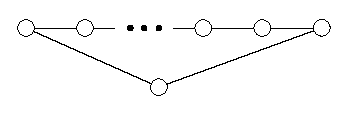
\includegraphics{table1_1(l).eps} & 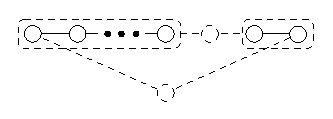
\includegraphics{table1_1(r).eps}
&  \\ \hline
$C_n$ & 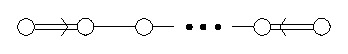
\includegraphics{table1_3(l).eps} & 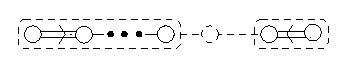
\includegraphics{table1_3(r).eps}
&  \\ \hline
$D_n$ & 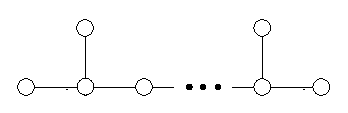
\includegraphics{table1_4(l).eps} & 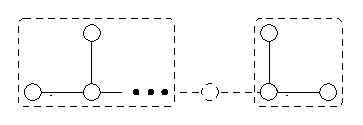
\includegraphics{table1_4(r).eps}
&  \\ \hline
\end{tabular}
}
\caption{Subalgebras $\af,\;\af_{\bot }$ for the classical series}
\end{table}


In the case of $B$ series the situation is different. The reason is that
here the subalgebra $\af_{\bot }$ may be larger than the one obtained
by elimination of the subdiagram of $\af$ and the adjacent nodes. The
subalgebras of the orthogonal pair,$\ \af$ and $\af_{\bot }$, must
not form a direct sum in $\frak{g}$ . It can be directly
checked that when $\frak{g}=B_{r}$ and $\af=B_{r_{\af}}$ the
orthogonal subalgebra is $\af_{\bot }=B_{r-r_{\af}}$. Consider the
injection $B_{r_{\af}}\rightarrow B_{r},\quad 1<r_{\af}<r$. By
eliminating the simple root $\alpha _{r_{\af}-1}=e_{r_{\af%
}-1}-e_{r_{\af}}$ one splits the extended Dynkin diagram of $B_{r}$
into the disjoint diagrams for $\af=B_{r_{\af}}$ and $D_{r-r_{%
\af}}$. But the system $\Delta _{\af_{\perp }}$ contains not only
the simple roots $\left\{ e_{1}-e_{2},e_{2}-e_{3},\ldots ,e_{r_{\af%
}-2}-e_{r_{\af}-1},e_{1}+e_{2}\right\} $ but also the root $e_{r_{\frak{%
a}}-1}$. Thus $\Delta _{\af_{\perp }}$ forms the subsystem of the type $%
B_{r-r_{\af}}$ and the orthogonal pair for the injection $B_{r_{\af%
}}\rightarrow B_{r}$ is $\left( B_{r_{\af}},B_{r-r_{\af}}\right) $%
. In the next Section the particular case of such orthogonal pair is
presented for the injection $B_{2}\rightarrow B_{4}$ (see Figure \ref
{fig:dynkin}).



The complete classification of regular subalgebras for affine Lie algebras
can be found in the recent paper \cite{1751-8121-41-36-365204}. From the complete
classification of maximal special subalgebras in classical Lie algebras \cite
{dynkin1952semisimple} we can deduce the following list of pairs of
orthogonal subalgebras $\af,\;\af_{\bot }$:
\begin{equation*}
\begin{array}{lll}
su(p)\oplus su(q) & \subset su(pq) &  \\
so(p)\oplus so(q) & \subset so(pq) &  \\
sp(2p)\oplus sp(2q) & \subset so(4pq) &  \\
sp(2p)\oplus so(q) & \subset sp(2pq) &  \\
so(p)\oplus so(q) & \subset so(p+q) & \mathrm{{for}\;p\;{and}\;q\;{odd}.}
\end{array}
\end{equation*}


\subsection{Algorithm for recursive computation of branching coefficients}

\label{sec:algorithm}

The recurrent relation (\ref{recurrent-relation}) allows us to formulate an
algorithm for recursive computation of branching coefficients. In this
algorithm there is no need to construct the module $L^{(\mu)}_{\frak{g}}$ or
any of the modules $L^{(\nu)}_{\af}$.

It contains the following steps:

\begin{enumerate}
\item  Construct the root system $\Delta _{\af}$ for the embedding $%
\af\rightarrow \frak{g}$.

\item  Select the positive roots $\alpha \in \Delta ^{+}$ orthogonal to the
roots in $\Delta _{\af}$ i.e. form the set $\Delta _{\bot }^{+}$.

\item  Construct the set $\Gamma _{\af\rightarrow \frak{g}}$ (\ref
{fan-defined}).

\item  Construct the set $\widehat{\Psi ^{(\mu )}}=\left\{ w (\mu +\rho
)-\rho ;\;w \in W\right\} $ of singular weights for the $\frak{g}$%
-module $L^{(\mu )}$.

\item  Select the weights $\left\{ \mu _{\widetilde{\af_{\perp }}%
}\left( w\right) =\pi _{\widetilde{\af_{\perp }}}\left[ w(\mu +\rho
)-\rho \right] -\mathcal{D}_{\af_{\perp }}\in \overline{C_{\widetilde{%
\af_{\perp }}}}\right\} $. Since the set $\Delta _{\bot }^{+}$ is fixed
we can easily check wether the weight $\mu _{\widetilde{\af_{\perp }}%
}\left( w\right) $ belongs to the main Weyl chamber $\overline{C_{\widetilde{%
\af_{\perp }}}}$ (by computing its scalar product with the roots from $%
\Delta _{\bot }^{+}$).

\item  For the weights $\mu _{\widetilde{\af_{\perp }}}\left( w\right) $
calculate the dimensions of the corresponding modules $\mathrm{\dim }\left(
L_{\widetilde{\af_{\perp }}}^{\mu _{\widetilde{\af_{\perp }}%
}\left( u\right) }\right) $.

\item  Calculate the anomalous branching coefficients in the main Weyl
chamber $\overline{C_{\af}}$ of the subalgebra $\af$ using the
recurrent relation (\ref{recurrent-relation}).
\end{enumerate}

When being interested in the branching coefficients for the embedding of a
finite-dimensional Lie algebra into an affine Lie algebra we can construct
the set of anomalous weights up to a required grade and use the steps
4-7 of the algorithm for each grade. We can also speed up the algorithm by
one-time computation of the representatives of the conjugate classes $%
W/W_{\afb }$.

The next section contains examples illustrating the application of this
algorithm.

\section{Branching for finite dimensional Lie algebras}
\label{sec:finite-dimens-lie}

\subsection{Regular embedding of $A_1$ into $B_2$}
\label{sec:regul-embedd-a_1}

Consider the regular embedding $A_1\to B_2$. Simple roots $\alpha_1, \alpha_2$ of $B_2$ are presented as the dashed vectors in the Figure \ref{fig:B2_A1}. We denote the corresponding Weyl reflections by $w_1, w_2$. The simple root $\beta = \alpha_1+2\alpha_2$ of $A_1$ is indicated as the grey vector.


\begin{figure}[p]
  \noindent\centering{
    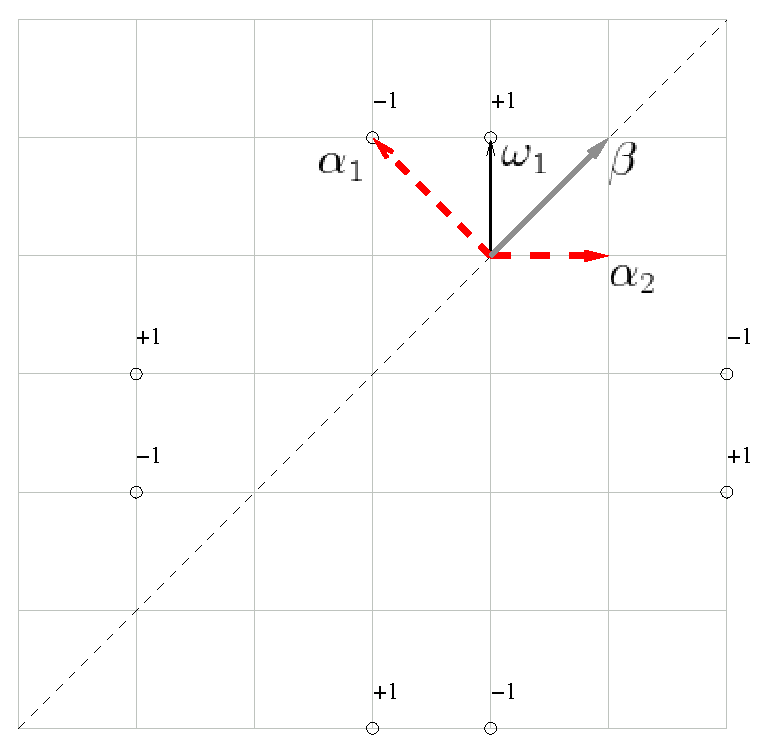
\includegraphics[width=80mm]{figure1.eps}
  }
  \caption{Regular embedding of $A_1$ into $B_2$. Simple roots $\alpha_1, \alpha_2$ of $B_2$ are presented as the dashed vectors.
    The simple root $\beta = \alpha_1+2\alpha_2$ of $A_1$ is indicated as the grey vector.
    The highest weight of the fundamental representation $L^{(1,0)=\omega_1}_{B_2}$ is shown by the black vector.
    The weights of the singular element $\Psi^{(\omega_1)}$ are indicated by the circles and the corresponding determinants $\epsilon(w)$ are shown.}
  \label{fig:B2_A1}

%\end{figure}
%\begin{figure}[pb]
  \noindent\centering{
    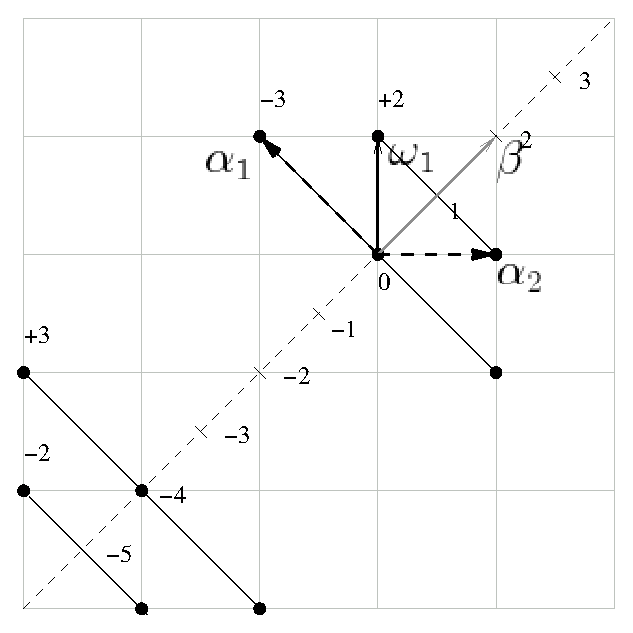
\includegraphics[width=80mm]{figure2.eps}
  }
  \caption{Regular embedding $A_1\subset B_2$. Simple roots $\alpha_1, \alpha_2$ of $B_2$ are presented as the dashed vectors.
    The simple root $\beta = \alpha_1+2\alpha_2$ of $A_1$ is indicated as the grey vector.
    The highest weight of the fundamental representation $L^{(1,0)=\omega_1}_{B_2}$ is shown by the black vector.  $\afb=A_1$-modules built on the weights of the singular element $\Psi^{(\omega_1)}$ are shown by dotted lines. The dimensions of these modules and the signs of the corresponding determinants $\epsilon(w)$ are shown near the anomalous weights. Fundamental weight coordinate of $\af=A_1$ is indicated on the weight subspace of $\af$. }
  \label{fig:B2_A1_2}
\end{figure}

Let's describe the reduction of the fundamental representation $L^{(1,0)=\omega_1}_{B_2}$ (the black vector in Figure \ref{fig:B2_A1}).

Circles indicate the weights of the singular element $\Psi^{(\omega_1)}$.
Now we are to factorise the Weyl group $W$ by $W_{\afb}=\left\{w_1\right\}$
and to construct the set $\left\{w(\mu+\rho)-\rho,\; w\in W_{\afb}\backslash W\right\}$.
In the Figure \ref{fig:B2_A1_2} the weights of the corresponding
$\left(\afb=A_1\right)$-modules
$L^{\pi_{\afb}(w(\mu+\rho))-\rho_{\afb}}_{\afb}$
are indicated. Projecting them onto the root space of the subalgebra $\af=A_1$
we get the anomalous weights and their multiplicities:
\begin{equation*}
  \label{eq:25}
  (1,2),\; (0,-3),\; (-4,3),\; (-5,-2).
\end{equation*}
For the set $\Gamma$ (using the definition \ref{fan-definition}) we have
\begin{equation*}
  \label{eq:22}
  \Gamma_{A_1\subset B_2}=\left\{ (1,2),\; (2,-1) \right\}.
\end{equation*}
Here the second component denotes the value of $s(\gamma)$.
Applying this fan inside the $\bar{C}^{(0)}_{\af}$ we get zeros for the weights
greater than the first anomalous vector $(1)$, here $k^{(1,0)}_1=2$. For the last weight in $\bar{C}^{(0)}_{\af}$ the formula (\ref{recurrent-relation}) gives
\begin{equation*}
  \label{eq:23}
  k^{(1,0)}_{0}=-1\cdot k^{(1,0)}_2 +2\cdot k^{(1,0)}_1 - 3\cdot \delta_{0,0} = 1.
\end{equation*}
The recurrence property defines the branching.

\subsection{Embedding of $B_2$ into $B_4$}
\label{sec:someth-high-dimens}
Consider the regular embedding $B_2 \longrightarrow B_4$.
The corresponding Dynkin diagrams are presented in the Figure \ref{fig:dynkin}.
\begin{figure}[h]
  \centering
  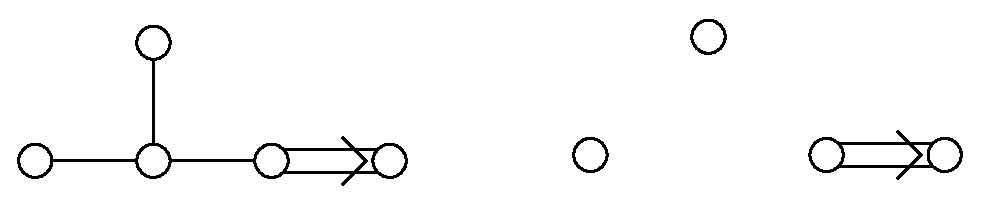
\includegraphics[width=50mm]{figure3.eps}
  \caption{The regular embedding $B_2\subset B_4$ described by dropping the node from the Dynkin diagram. Note, that $\afb$ is equal to $B_2$, not to $A_1\oplus A_1$ seen at the diagram.}
  \label{fig:dynkin}
\end{figure}

\begin{figure}[pt]
  \centering
    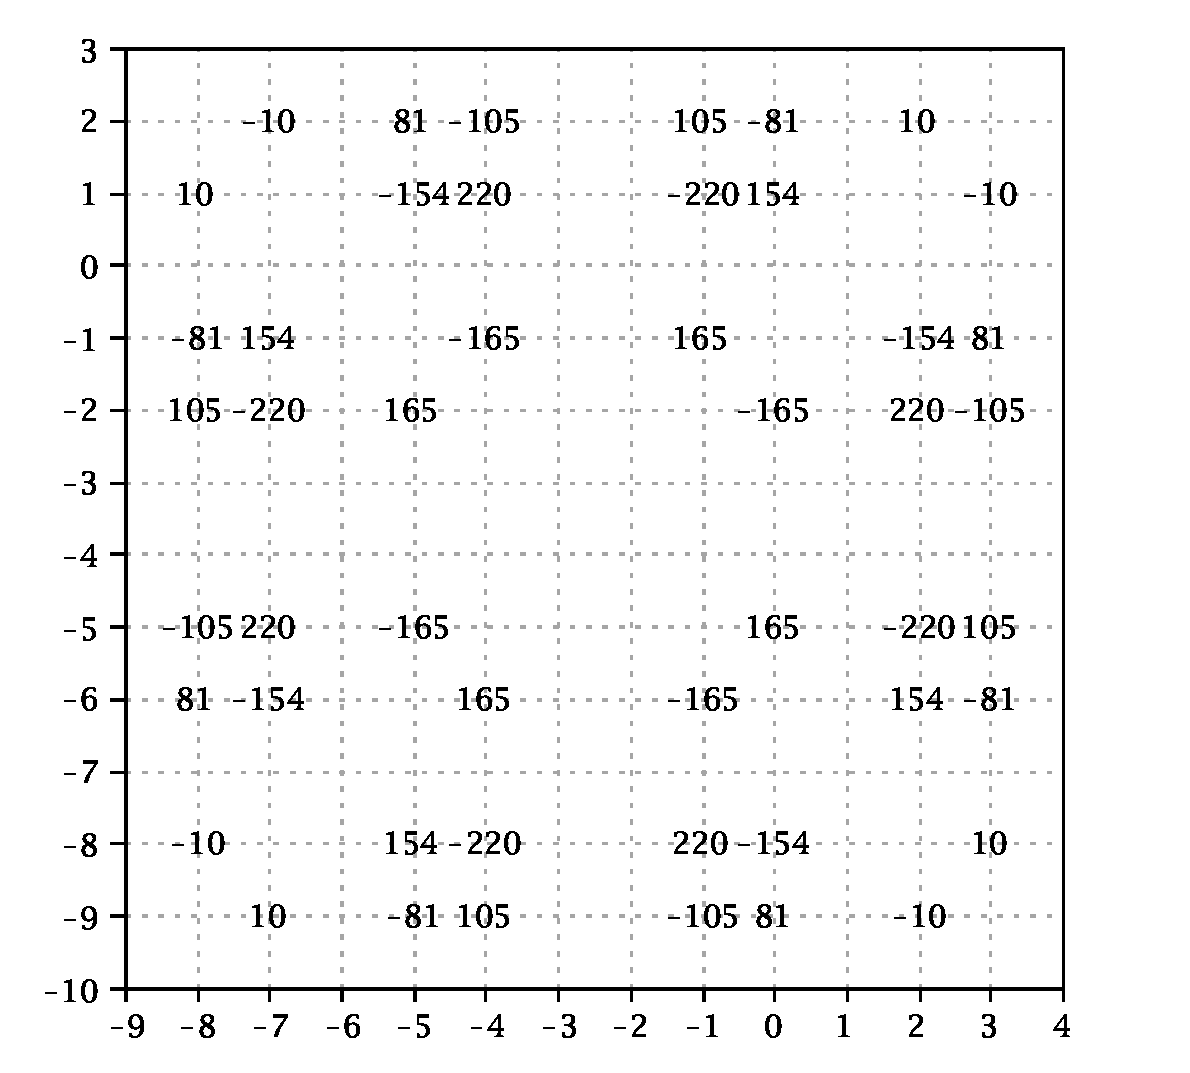
\includegraphics[width=100mm,height=90mm]{figure4.eps}
  \caption{Projected singular weights of $-\frac{1}{s(\gamma_0)}\pi_{B_2}\left(\hat \Psi^{(0,1,0,2)}_{B_4}\right)$
  with the dimensions of the corresponding $\afb=B_2$-modules.}
  \label{fig:B4B2anom}

%\end{figure}
%
%\begin{figure}[pb]
  \centering
  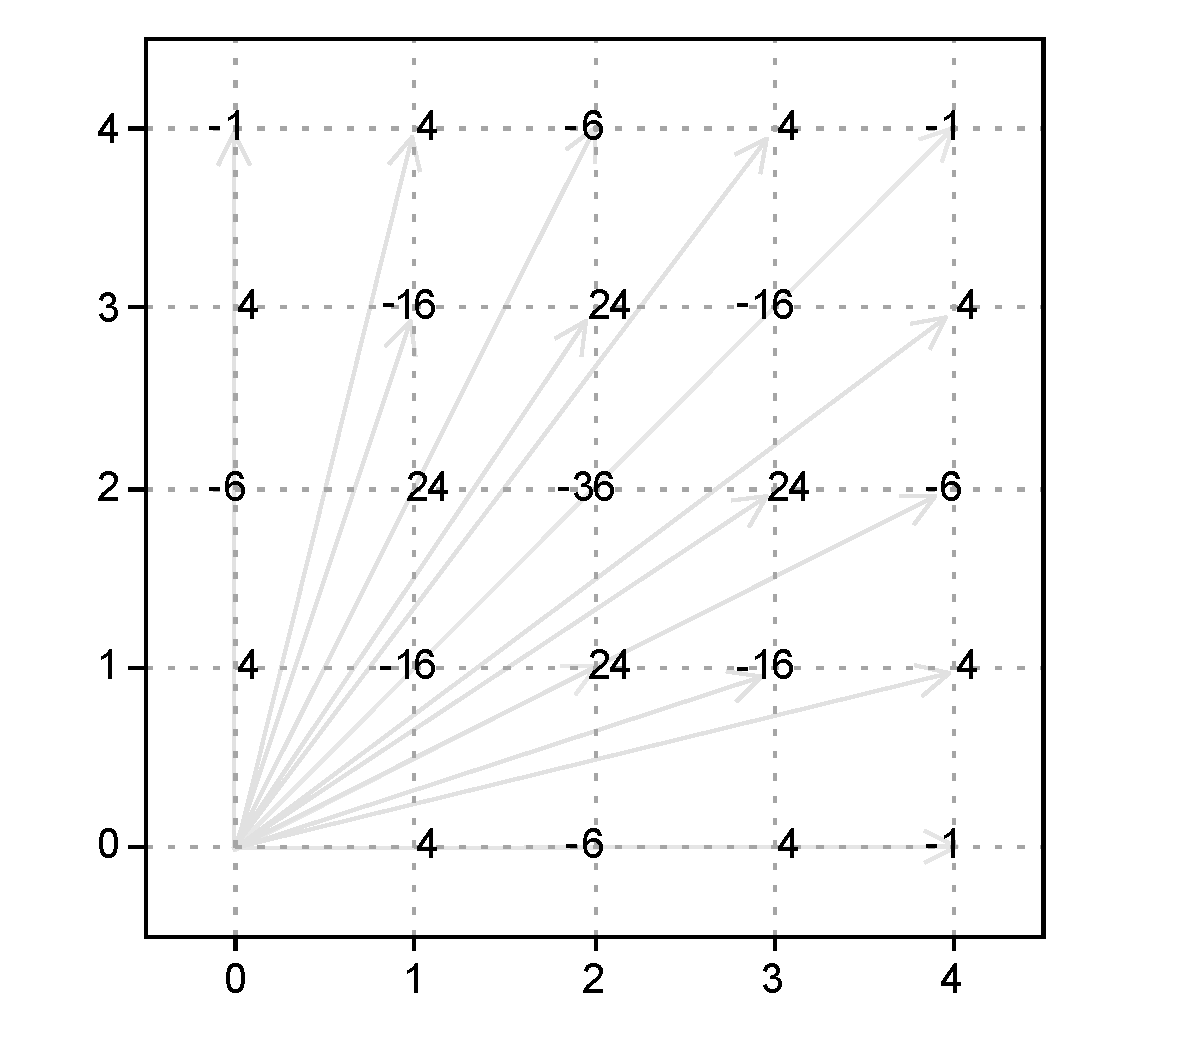
\includegraphics[height=80mm]{figure5.eps}
  \caption{The fan $\Gamma_{B_2\subset B_4}$ for $B_2\subset B_4$. The values $s(\gamma+\gamma_0)$ are shown in the corresponding weights $\gamma$.}
  \label{fig:B4B2Fan}
\end{figure}

In the orthogonal basis $\left\{e_1,\dots,e_4\right\}$ the simple roots and the positive roots of $B_4$ are
\begin{equation*}
  \label{eq:8}
 S_{B_4}= \{e_1 - e_2,\; e_2 - e_3,\; e_3 - e_4,\; e_4\}
\end{equation*}
\begin{eqnarray*}
  \label{eq:19}
 \Delta^+_{B_4}=\left\{ (e_1 - e_2,\; e_2 - e_3,\; e_3 - e_4,\; e_4,\; e_1 - e_3,\; e_2 - e_4,\; e_3 + e_4,\; e_3,\; e_1 - e_4,\;\right.\\
 \left. e_2 + e_4,\; e_2,\; e_1 + e_4,\; e_2 + e_3,\; e_1,\; e_1 + e_3,\; e_1 + e_2\right\}
\end{eqnarray*}
Correspondingly for the embedded subalgebra $\af=B_2$ we have
\begin{equation*}
  \label{eq:26}
 S_{B_2}=\{e_3-e_4,e_4\}
\end{equation*}
and
\begin{equation*}
  \label{eq:27}
 \Delta^{+}_{\afb}= \left\{e_1-e_2,e_1+e_2,e_1,e_2\right\}
\end{equation*}
is the set of positive roots for the algebra $\afb=B_2$.

Using the definition (\ref{fan-defined}) we obtain the fan
$\Gamma_{B_2\subset B_4}$ with the corresponding values $s(\gamma+\gamma_0)$,
depicted in the Figure \ref{fig:B4B2Fan}.


Consider the $B_4$-module $L^{\mu}$ with the highest weight $\mu=(0,1,0,2)=2
e_1 + 2 e_2 + e_3 + e_4$; $\mathrm{dim}(L^{(0,1,0,2)})=2772$.
To find the branching coefficients we need to compute the anomalous weights of
$L^{\mu}_{B_4}$, select the weights belonging to $\bar{C}^{\left( 0 \right)}_{\afb}$
and compute the dimensions of the corresponding $\afb$-modules.
The set of the anomalous weights $\left\{ w(\mu+\rho)-\rho,\; w\in W\right\}$
contains 384 vectors.

We are to select the weights $\psi \in w(\mu+\rho)$  with the property
$\pi_{\afb} \left(  \psi \right) \in \bar{C}^{\left( 0 \right)}_{\afb}$.
It means that the scalar product of these weights with all the roots in $\Delta^{+}_{\afb}$ is nonnegative.

To compute the dimensions of the corresponding
$\afb$-modules we need to project each selected weight
onto the root space $\Delta^{+}_{\afb}$, subtract
$\rho_{\afb}$ and apply the Weyl dimension formula. The result is shown in the Figure \ref{fig:B4B2anom}.

Applying the recurrent relation (\ref{recurrent-relation}) we obtain the
following branching coefficients:
\begin{eqnarray*}
  \label{eq:24}
  \pi_{\af} \left(ch L^{(0,1,0,2)}_{B_4}\right) = 6 \; ch L^{(0,0)}_{B_2}+ 60
  \; ch L_{B_2}^{(0,2)}+ 30 \; ch L_{B_2}^{(1,0)}+ 19 \; ch L_{B_2}^{(2,0)}+\\
  40 \; ch L_{B_2}^{(1,2)}+ 10 \; ch L_{B_2}^{(2,2)}.
\end{eqnarray*}
%\newpage
\section{Applications to the conformal field theory}
\label{sec:phys-appl}

\subsection{Conformal embeddings}
\label{sec:conformal-embeddings}

Branching coefficients for an embedding of affine Lie algebra into
affine Lie algebra can be used to construct modular invariant
partition functions for Wess-Zumino-Novikov-Witten models in conformal field theory
(\cite{difrancesco1997cft}, \cite{Walton:1999xc}, \cite{walton1989conformal}, \cite{schellekens1986conformal}).
In these models current algebras are affine Lie algebras.

The modular invariant partition function is crucial for the conformal theory to be valid
on the torus and higher genus Riemann surfaces. It is important for the applications of
CFT to the string theory and to the critical phenomena description.

The simplest modular-invariant partition function has the diagonal form:
\begin{equation*}
  \label{eq:34}
   Z(\tau)=\sum_{ \mu\in P^{+}_{\mathfrak{g}}} \chi_{\mu}(\tau)\bar \chi_{\mu}(\bar \tau)
\end{equation*}
Here the sum is over the set of the highest weights of integrable modules in a WZW-model
and $\chi_{\mu}(\tau)$ are the normalized characters of these modules.

To construct the nondiagonal modular invariants is not an easy problem,
although for some models the complete classification of modular invariants is known \cite{1994hepthGannon,1995JMPGannon}.

Consider the Wess-Zumino-Witten model with the affine Lie algebra $\af$.
Nondiagonal modular invariants for this model can be constructed from the diagonal
invariant if there exists an affine algebra $\mathfrak{g}$ such that $\af\subset\mathfrak{g}$.
Then we can replace the characters of the $\mathfrak{g}$-modules in the diagonal
modular invariant partition function (\ref{eq:36})
by the decompositions
\begin{equation*}
  \label{eq:32}
\sum_{\nu \in P^{+}_{\af}}b^{(\mu)}_{\nu} \chi_{\nu}
\end{equation*}
containing the modified characters $\chi_{\nu}$ of the corresponding $\af$-modules.
Thus we obtain the nondiagonal modular-invariant  partition function for the theory with
the current algebra $\af$,
\begin{equation}
  \label{eq:36}
   Z_{\af}(\tau)=\sum_{ \nu,\lambda\in P^{+}_{\af}} \chi_{\nu}(\tau)M_{\nu\lambda}\bar \chi_{\lambda}(\bar \tau).
\end{equation}

The effective reduction procedure is crucial for this construction.
The embedding is required to preserve the conformal invariance.
Let $X^{\alpha_j}_{-n_j}$ and $\tilde{X}^{\alpha'_j}_{-n_j}$ be the lowering generators for
$\mathfrak{g}$ and for $\af\subset\mathfrak{g}$ correspondingly.
Let $\pi_{\af}$ be the projection operator of
$\pi_{\af}:\mathfrak{g}\longrightarrow \af$.
In the theory attributed to $\mathfrak{g}$ with the vacuum $\left|\lambda\right>$
the states can be described as
\begin{equation*}
  \label{eq:109}
  X^{\alpha_1}_{-n_1}X^{\alpha_2}_{-n_2}\dots\left|\lambda\right>\quad n_1\geq n_2\geq \dots>0.
\end{equation*}
And for the sub-algebra $\af$ the corresponding states are
\begin{equation*}
  \label{eq:110}
  \tilde{X}^{\alpha'_1}_{-n_1}\tilde{X}^{\alpha'_2}_{-n_2}\dots\left|\pi_{\af}(\lambda)\right>.
\end{equation*}
The $\mathfrak{g}$-invariance of the vacuum entails its $\af$-invariance,
but this is not the case for the energy-momentum tensor. So the energy-momentum tensor of the larger theory
should contain only the generators $\tilde{X}$. Then the relation
\begin{equation}
  \label{eq:2}
  T_{\mathfrak{g}}(z)=T_{\af}(z)
\end{equation}
leads to the equality of the central charges
\begin{equation*}
  \label{eq:33}
  c(\mathfrak{g})=c(\af)
\end{equation*}
and to the equation
\begin{equation}
  \label{eq:111}
  \frac{k\;\mathrm{dim}\,\mathfrak{g}}{k+g}=\frac{x_e k\; \mathrm{dim}\,\af}{x_ek+a}.
\end{equation}
Here $x_e$ is the so called "embedding index":
$x_e=\frac{\left|\pi_{\mathfrak{a}} \Theta\right|^2}{\left|\Theta_{\mathfrak{a}}\right|^2}$
with $\Theta$, $\Theta_{\mathfrak{a}}$ being the highest roots of
$\mathfrak{g}$ and $\mathfrak{a}$
while $g$  and $a$ are the  corresponding dual Coxeter numbers.

It can be demonstrated that the solutions of the equation (\ref{eq:111}) exist only
for the level $k=1$ \cite{difrancesco1997cft}.

The complete classification of conformal embeddings is given in \cite{schellekens1986conformal}.

The relation (\ref{eq:111}) and the asymptotics of the branching functions can be used
to prove the finite reducibility theorem \cite{kac1988modular}.
It states that for the conformal embedding  $\af\subset\mathfrak{g}$
only finite number of branching coefficients have nonzero values.

\begin{mynote} The orthogonal subalgebra $\afb$ is always empty for the conformal embeddings $\af\subset \mathfrak{g}$.
\begin{proof}
Consider the modes expansion of the energy-momentum tensor
\begin{equation*}
\label{eq:47}
  T(z)=\frac{1}{2(k+h^v)}\sum_n z^{-n-1}L_n.
\end{equation*}
The modes $L_n$ are constructed as combination of normally-ordered products of the generators of $\mathfrak{g}$,
\begin{equation*}
\label{eq:48}
  L_n=\frac{1}{2(k+h^v)}\sum_{\alpha}\sum_m:X^{\alpha}_m X^{\alpha}_{n-m}: \; .
\end{equation*}
In the case of a conformal embedding energy-momentum tensors are to be equal (\ref{eq:2}).

The substitution of the generators of $\af$  in terms of the generators of $\mathfrak{g}$ into these combinations  should give the energy-momentum tensor $T_{\mathfrak{g}}$. But if the set of the generators $\Delta_{\afb}$ is not empty this is not possible, since $T_{\mathfrak{g}}$ contains the combinations of the generators $X^{\alpha}_n, \; \alpha\in \Delta_{\afb}$.
\end{proof}
\end{mynote}
\subsubsection{Special embedding $\hat{A}_1\subset\hat{A}_2$.}
\label{sec:spec-embedd-hata_1s}

Consider the case where both $\mathfrak{g}$ and $\af$ are affine Lie algebras:
$\hat{A}_1 \longrightarrow \hat{A}_2$ and the injection is the affine extension of the
special injection $A_1 \longrightarrow A_2$ with the embedding index $x_e=4$.
As far as the $\mathfrak{g}$-modules to be considered are of level one,
the $\mathfrak{g}$-modules will be of level $\tilde{k}=kx_e=4$.

There exist three level one fundamental weights in the weight space of $\hat{A}_2$.
It is easy to see that the set $\Delta_{\afb}$ is empty and the subalgebra $\afb=0$.

Using the definition (\ref{fan-defined})  we construct the fan $\Gamma_{\hat A_1\to\hat A_2}$
and the function $s(\gamma+\gamma_0)$ (see the Figure \ref{fig:AffineA2A1Fan}).

\begin{figure}[h!bt]
  \centering
  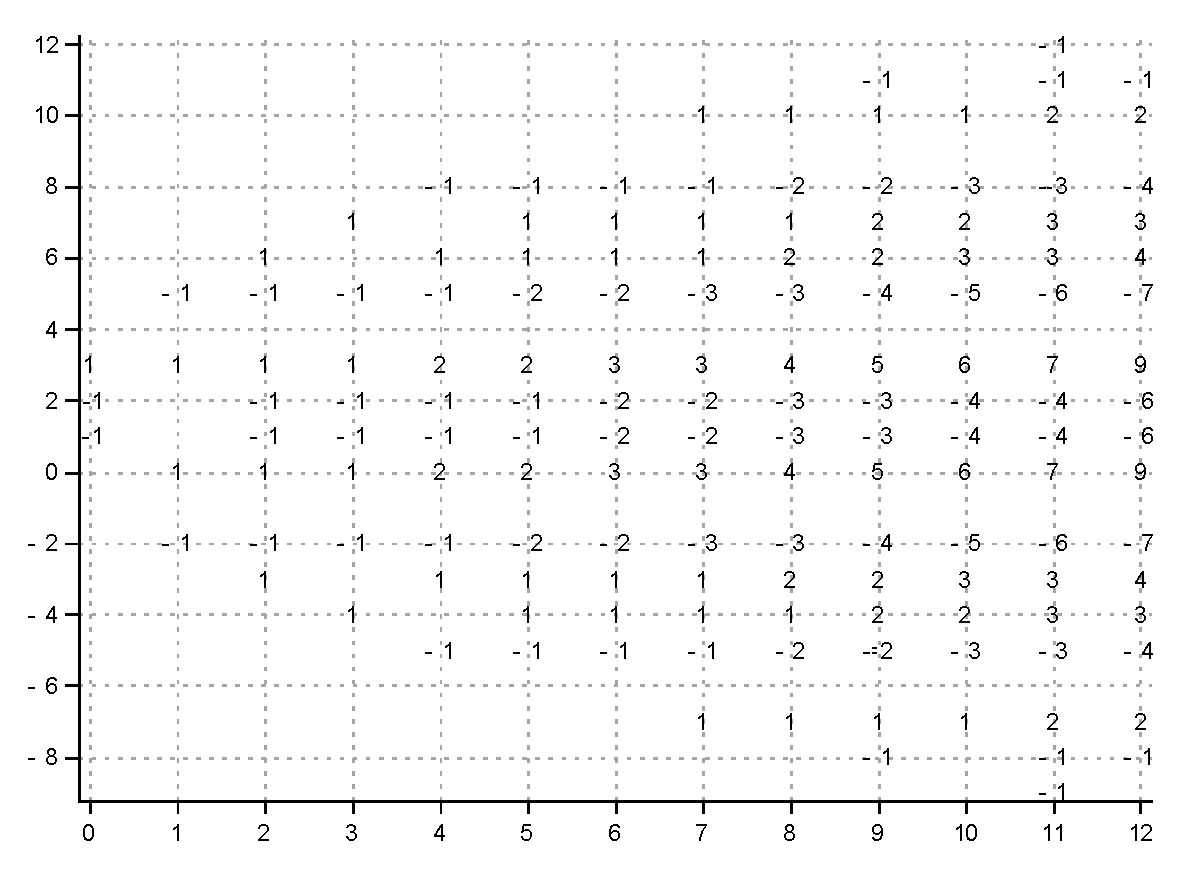
\includegraphics[width=135mm]{figure6.eps}

  \caption{The fan $\Gamma_{\hat{A_1}\longrightarrow \hat{A_2}}$ for $\hat{A_1}\longrightarrow \hat{A_2}$. Values of  $s(\gamma+\gamma_0)$ are shown for the weights $\gamma\in \Gamma_{\hat{A_1}\longrightarrow \hat{A_2}}$}
  \label{fig:AffineA2A1Fan}
\end{figure}

Let us consider the module $L^{\omega_0=(0,0;1;0)}$. Here we use the (finite part; level; grade)
presentation of the highest weight and the finite part
coordinates are the Dynkin indices (see section(\ref{sec:notation})).

The set $\widehat{\Psi^{(\omega_0)}}$  is depicted in the Figure
\ref{fig:affine_A2_anom_point} up to the sixth grade.

\begin{figure}[h!tb]
%  \hspace*{-2cm}
  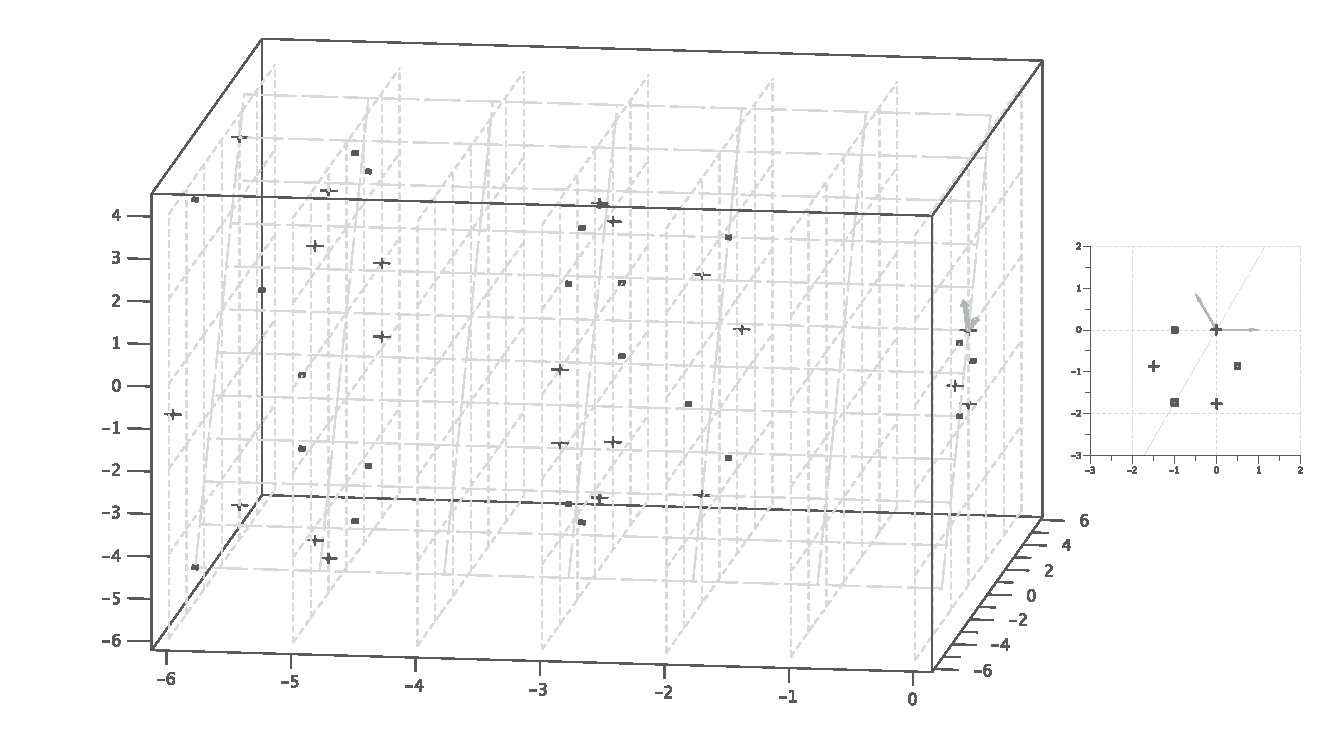
\includegraphics[width=140mm]{figure7.eps}
  \caption{The anomalous weights of the module $L_{\hat{A_2}}^{\omega_0}=L^{(0,0;1;0)}_{\hat{A_2}}$. The weights $w (\omega_0+\rho)-\rho$ are marked by crosses when $\epsilon(w)=1$ and
by diamond when $\epsilon(w)=-1$. Simple roots of the classical subalgebra $A_2$ are
grey and the grey diagonal plane corresponds to the Cartan subalgebra of
the embedded algebra $\hat{A}_1$.}
  \label{fig:affine_A2_anom_point}
\end{figure}

The next step is to project the anomalous weights to $P_{\hat A_1}$.
The result is presented in the Figure \ref{fig:AffineA2_A1_anom_proj} up to the twelfth grade.
\begin{figure}[h!tb]
  \centering
  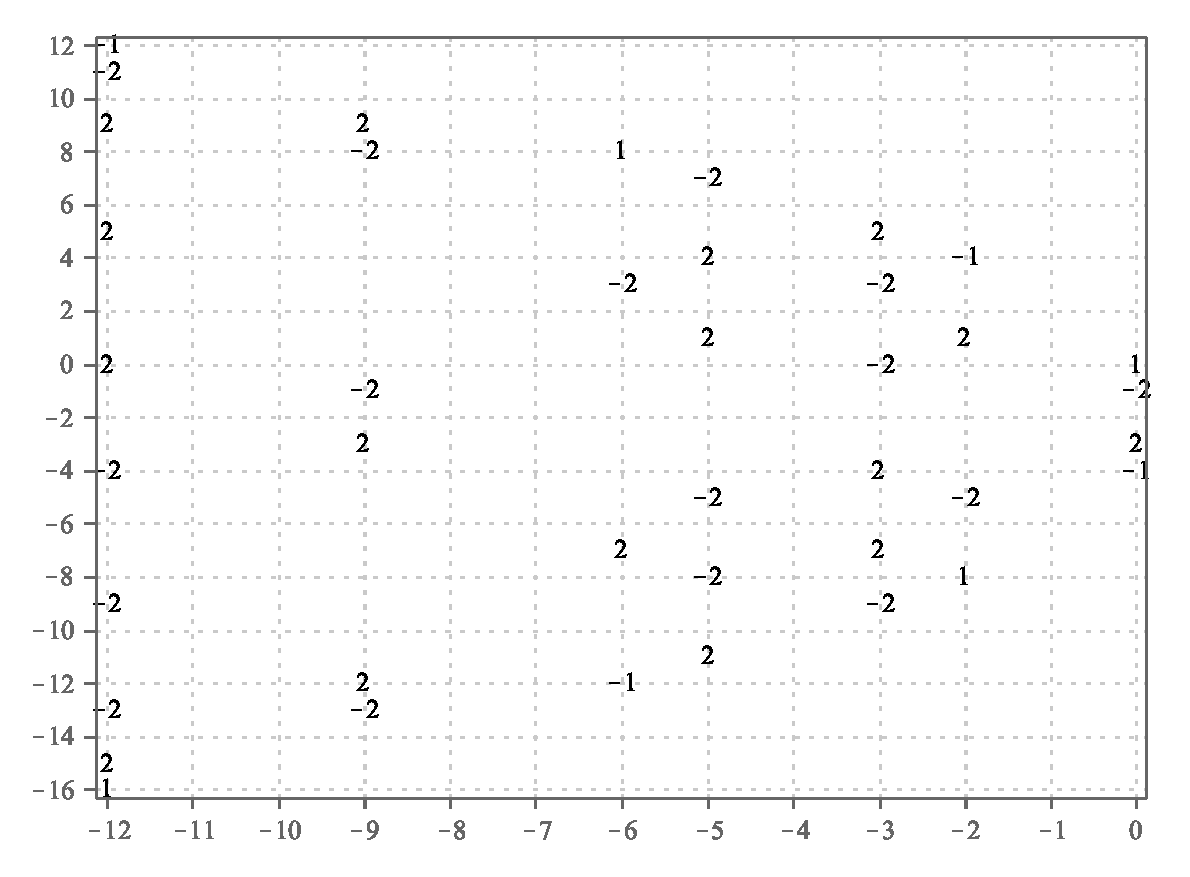
\includegraphics[width=130mm]{figure8.eps}
  \caption{Projected anomalous weights of $L^{(0,0;1;0)}_{\hat{A_2}}$. The multiplicities of projected weights and the corresponding signs are shown. }
  \label{fig:AffineA2_A1_anom_proj}
\end{figure}


Using the recurrent relation for the anomalous branching coefficients
we get the result presented in Figure \ref{fig:AffineA2_A1_branching}.
\begin{figure}[h!tb]
  \centering
  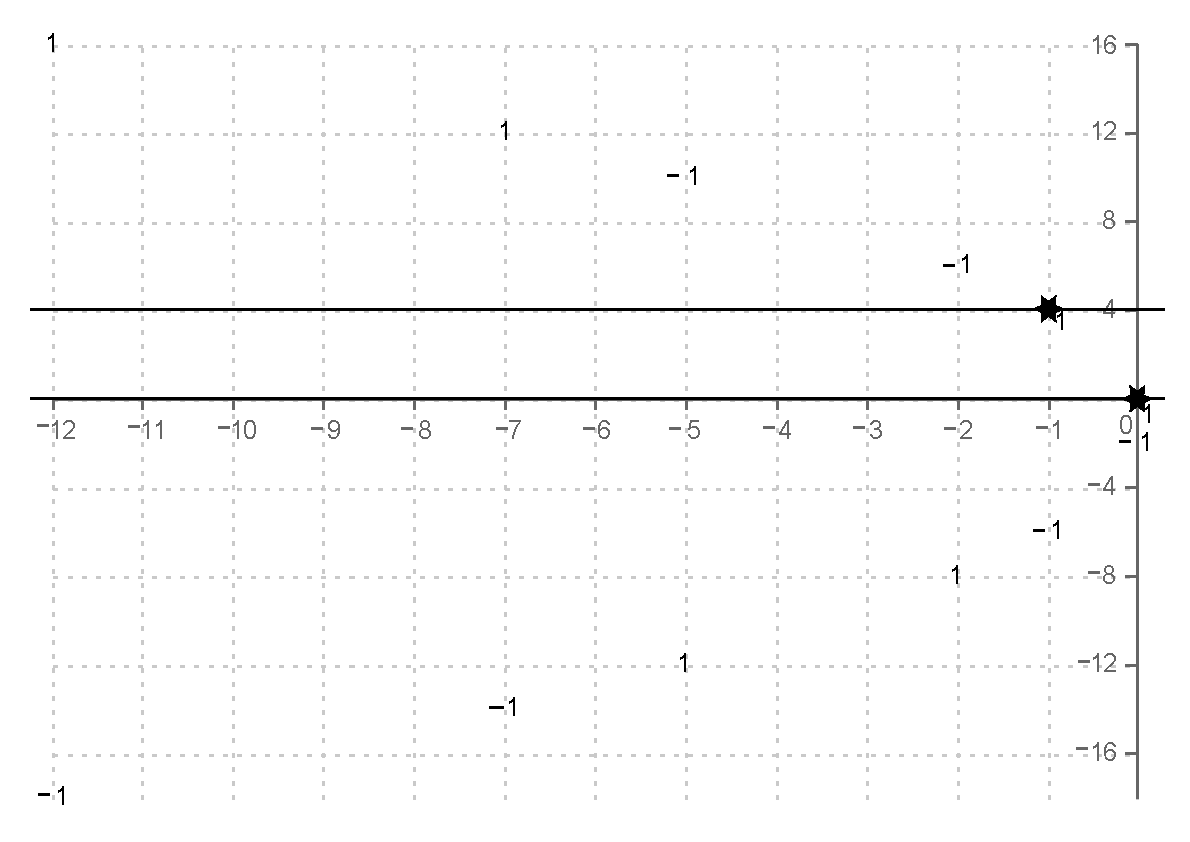
\includegraphics[width=130mm]{figure9.eps}
  \caption{Anomalous branching coefficients for $\hat{A_1}\subset \hat{A_2}$. The boundaries  of the main Weyl chamber $\bar{C}_{\hat{A}_1}$
 are indicated by the black lines. Two nonzero anomalous weights in the main Weyl chamber are marked by stars. Both weights have multiplicity 1, so the branching coefficients are equal to 1.}
  \label{fig:AffineA2_A1_branching}
\end{figure}
Inside the Weyl chamber $\bar{C}_{\hat{A}_1}$
(its boundaries are indicated in the Figure \ref{fig:AffineA2_A1_branching})
there are only two nonzero anomalous weights and both have multiplicity 1.
These are the highest weights of $\af$-submodules and their branching
coefficients. So the finite reducibility theorem holds and we get the decomposition
\begin{equation*}
  \label{eq:43}
  L^{(0,0;1;0)}_{\hat{A_2}\downarrow \hat{A_1}}= L_{\hat{A_1}}^{(0;4;0)}\oplus L_{\hat{A_1}}^{(4;4;0)}.
\end{equation*}

For the other irreducible modules of level one  we get the trivial
branching
\begin{equation*}
  \label{eq:44}
   L^{(1,0;1;0)}_{\hat{A_2}\downarrow \hat{A_1}}= L_{\hat{A_1}}^{(2;4;0)},\\
   L^{(0,1;1;0)}_{\hat{A_2}\downarrow \hat{A_1}}= L_{\hat{A_1}}^{(2;4;0)}.
\end{equation*}

Using these results the modular-invariant partition function is easily found,
\begin{equation*}
  \label{eq:45}
  Z=\left|\chi_{(4;4;0)}+\chi_{(0;4;0)}\right|^2+2\chi_{(2;4;0)}^2.
\end{equation*}

\subsection{Coset models}
\label{sec:coset-models}

Coset models \cite{Goddard198588} tightly connected with the gauged WZW-models are actively studied
in string theory, especially in string models on anti-de-Sitter space
\cite{Maldacena:2000hw,Maldacena:2000kv,Maldacena:2001km,Maldacena:2001ky,Aharony:1999ti}.
The characters in coset models are proportional to the branching functions,
\begin{equation}
  \label{eq:31}
  \chi^{(\mu)}_{\nu}(\tau)=e^{2\pi i \tau (m_{\mu}-m_{\nu})} b^{(\mu)}_{\nu}(\tau),
\end{equation}
with
\begin{equation*}
  \label{eq:46}
  m_{\mu}=\frac{\left|\mu+\rho\right|^2}{2(k+g)}-\frac{\left|\rho\right|^2}{2g}.
\end{equation*}
The problem of the branching functions construction in the coset models was considered
in  \cite{Dunbar:1992gh}, \cite{Hwang:1994yr}, \cite{lu1994branching}.

Let us return to the example \ref{sec:regul-embedd-a_1} and consider the affine extension of the injection
$A_1 \longrightarrow B_2$.
Since this embedding is regular and $x_e=1$, the subalgebra modules and the initial module are of the same level.
The set $\Delta^{+}_{\afb}$ of the orthogonal positive roots with the zero projection
on the root space of the subalgebra $\hat{A_1}$ is the same as in the finite-dimensional case.

Using the definition (\ref{fan-defined}) we get the fan
$\Gamma_{\hat{A_1} \longrightarrow  \hat{B_2} }$
with the corresponding values $s(\gamma+\gamma_0)$ (see the Figure \ref{fig:AffineB2A1Fan}).
We restricted the computation to the twelfth grade.
\begin{figure}[h!bt]
  \centering
  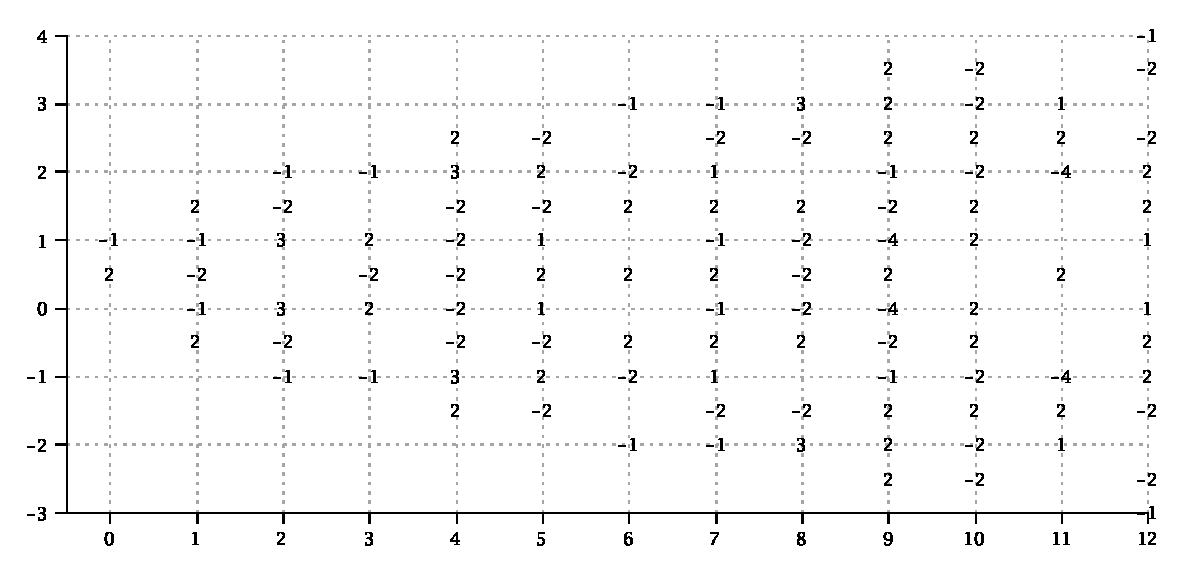
\includegraphics[width=135mm]{figure10.eps}
  \caption{The fan $\Gamma_{\hat{A_1}\longrightarrow \hat{B_2}}$ for $\hat{A_1}\longrightarrow \hat{B_2}$. Values of  $s(\gamma+\gamma_0)$ are shown for the weights $\gamma\in \Gamma_{\hat{A_1}\longrightarrow \hat{B_2}}$}
  \label{fig:AffineB2A1Fan}
\end{figure}


Consider the level one module $L^{\left( 1,0;1;0 \right)}_{\hat{B_2}}$  with the highest weight $\omega_1=(1,0;1;0)$,
where the finite part coordinates are in the orthogonal basis $e_1,e_2$.
The set of anomalous weights for this module up to the sixth grade is presented in the Figure \ref{fig:affine_B2_anom_point}.
In the grade zero it is exactly the set of the anomalous weights for the embedding of
the classical Lie algebras $A_1\subset B_2$ that can be seen in the  Figure \ref{fig:B2_A1}.

\begin{figure}[h!tb]
%  \hspace*{-2cm}
  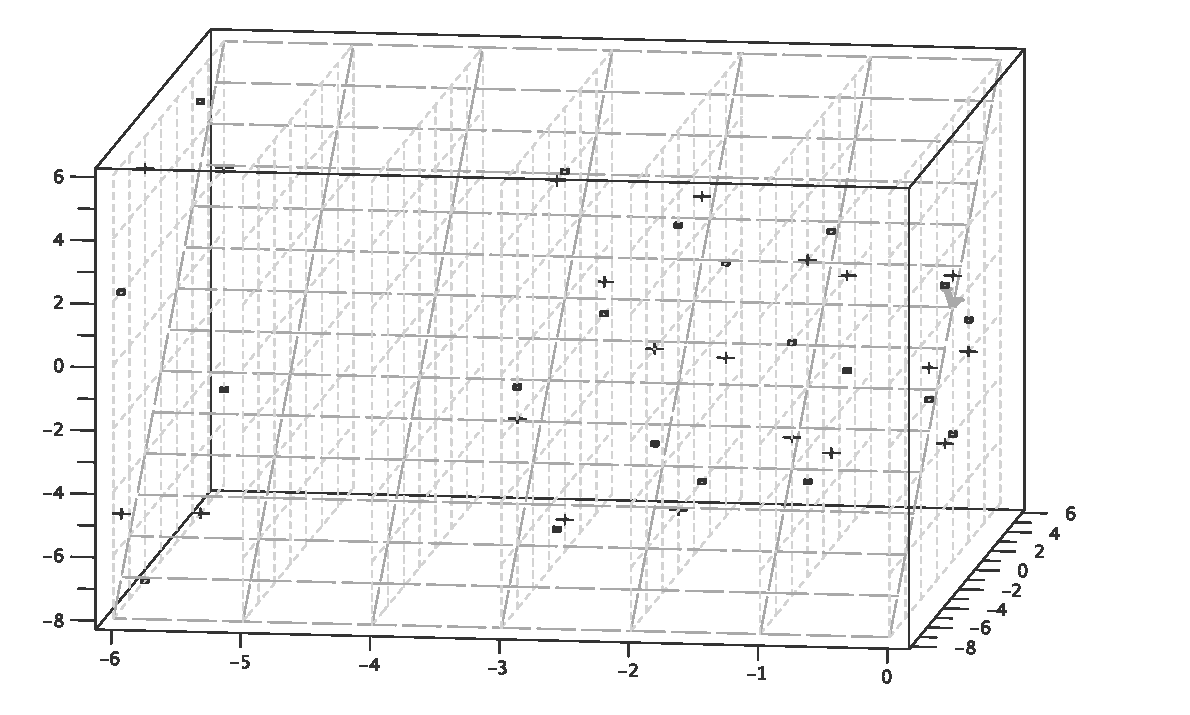
\includegraphics[width=140mm]{figure11.eps}
  \caption{The anomalous weights of $L^{(1,0;1;0)}_{\hat B_2 }$.
  The weights in the zero grade can be seen in the Figure \ref{fig:B2_A1}. The weights $w (\omega_1+\rho)-\rho$ are marked by crosses if $\epsilon(w)=1$ and by circles otherwise.
Simple roots of the classical subalgebra $B_2$ are grey and grey diagonal plane corresponds to the Cartan subalgebra
of the embedded algebra $\hat{A}_1$.}
  \label{fig:affine_B2_anom_point}
\end{figure}

According to the algorithm \ref{sec:algorithm} we project the anomalous weights to
$P_{\hat{A_1}}$ and find the dimensions of the corresponding
$\afb$-modules $L^{\pi_{\afb}(w(\mu+\rho))-\rho_{\afb}}_{\afb}$.
The result is presented in the Figure
\ref{fig:AffineB2_A1_anom_proj} up to the twelfth grade.
\begin{figure}[h!tb]
  \centering
  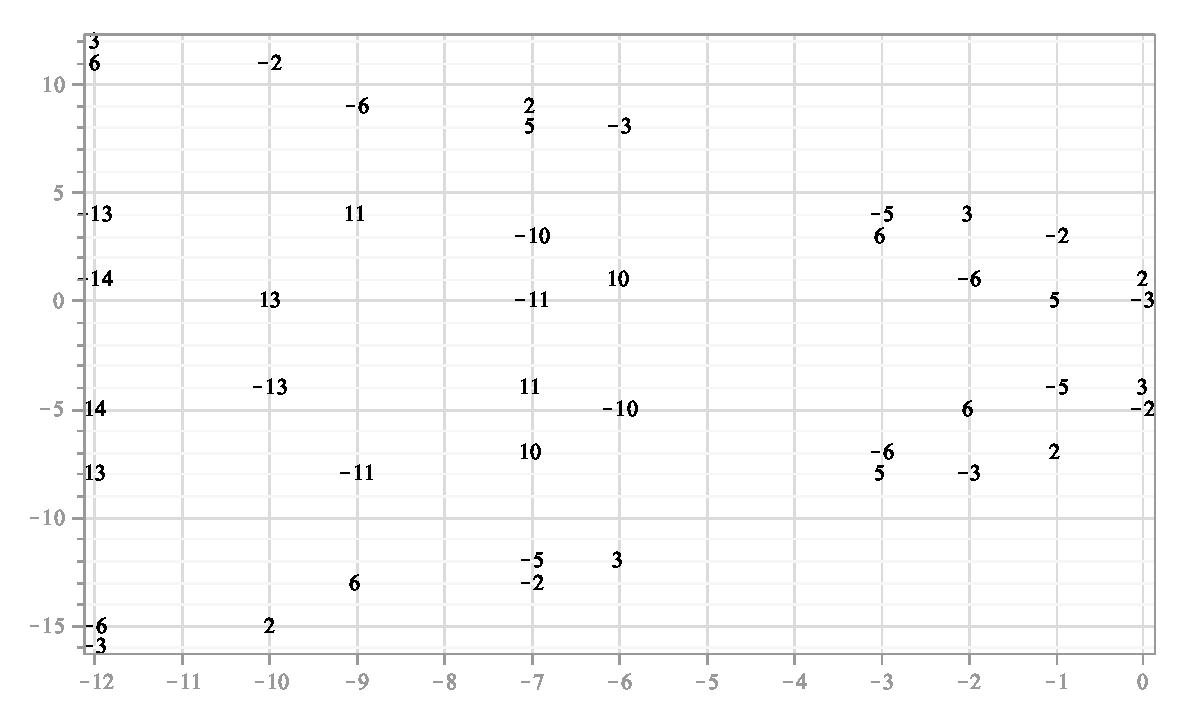
\includegraphics[width=120mm]{figure12.eps}
  \caption{The projected anomalous weights $\pi_{\hat A_1}\left(\Psi^{(1,0;1;0)}_{\hat B_2}\right)$. The dimensions of the corresponding $\afb=A_1$-modules with the signs $\epsilon(w)$ are shown.}
  \label{fig:AffineB2_A1_anom_proj}
\end{figure}

Notice that here the lowest weight  $\gamma_0$ of the fan  is zero, since we have excluded all the roots of $\Delta^{+}_{\afb}$ from the defining relation (\ref{fan-defined}).

\begin{figure}[h!bt]
  \centering
  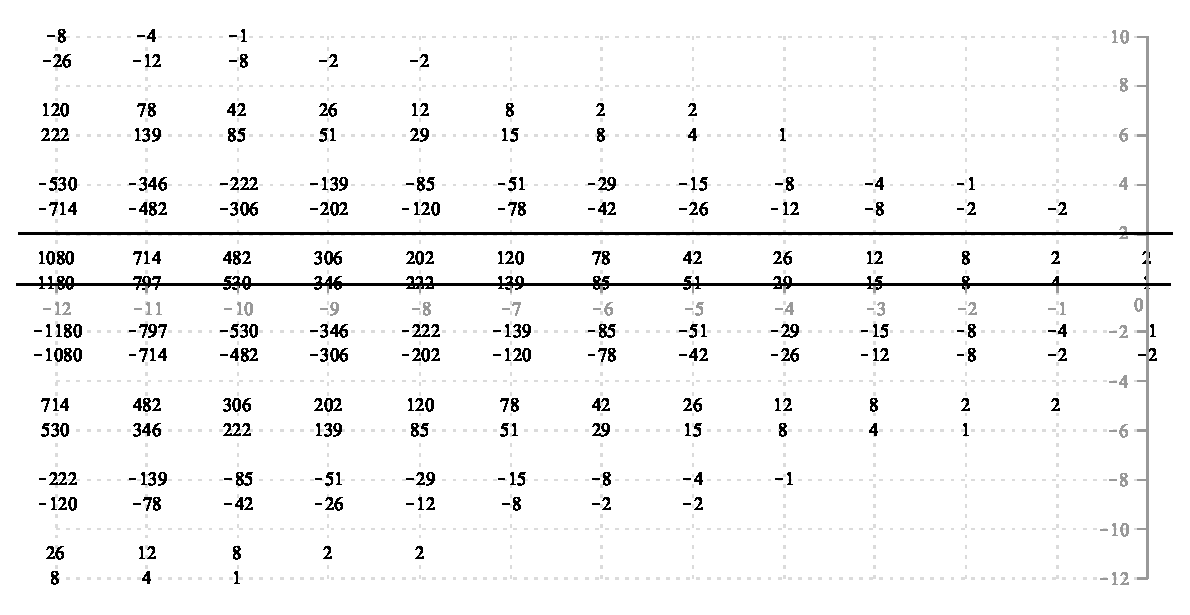
\includegraphics[width=120mm]{figure13.eps}
  \caption{Anomalous branching coefficients for $\hat{A_1}\subset \hat{B_2}$.  The boundaries  of the main Weyl chamber $\bar{C}_{\hat{A}_1}$
 are indicated by the black lines. The anomalous branching coefficients inside the main Weyl chamber are equal to the branching coefficients of the embedding $\hat{A_1}\longrightarrow \hat{B_2}$.}
  \label{fig:AffineB2_A1_branching}
\end{figure}

The multiplicities of the weights inside the  Weyl chamber
$\bar{C}^{\left( 0 \right)}_{\hat{A_1}}$
are the branching coefficients (up to the twelfth grade),
\begin{eqnarray*}
  \label{eq:28}
  L^{\omega_1}_{\hat{B_2}\downarrow \hat{A_1}}=2 L_{\hat{A_1}}^{\omega_1}\oplus 1 L_{\hat{A_1}}^{\omega_0}\oplus 4 L_{\hat{A_1}}^{\omega_0-\delta}\oplus\\
    2 L_{\hat{A_1}}^{\omega_1-\delta}\oplus 8 L_{\hat{A_1}}^{\omega_0-2\delta}\oplus
    8 L_{\hat{A_1}}^{\omega_1-2\delta}\oplus 15 L_{\hat{A_1}}^{\omega_0-3\delta}\oplus\\
    12 L_{\hat{A_1}}^{\omega_1-3\delta}\oplus 26 L_{\hat{A_1}}^{\omega_1-4\delta}\oplus
    29 L_{\hat{A_1}}^{\omega_0-4\delta}\oplus 51 L_{\hat{A_1}}^{\omega_0-5\delta}\oplus\\
    42 L_{\hat{A_1}}^{\omega_1-5\delta}\oplus 78 L_{\hat{A_1}}^{\omega_1-6\delta}\oplus
    85 L_{\hat{A_1}}^{\omega_0-6\delta}\oplus 120 L_{\hat{A_1}}^{\omega_1-7\delta}\oplus\\
    139 L_{\hat{A_1}}^{\omega_0-7\delta}\oplus 202 L_{\hat{A_1}}^{\omega_1-8\delta}\oplus
    222 L_{\hat{A_1}}^{\omega_0-8\delta}\oplus 306 L_{\hat{A_1}}^{\omega_1-9\delta}\oplus\\
    346 L_{\hat{A_1}}^{\omega_0-9\delta}\oplus 530 L_{\hat{A_1}}^{\omega_0-10\delta}\oplus
    482 L_{\hat{A_1}}^{\omega_1-10\delta}\oplus 714 L_{\hat{A_1}}^{\omega_1-11\delta}\oplus\\
    797 L_{\hat{A_1}}^{\omega_0-11\delta}\oplus 1080 L_{\hat{A_1}}^{\omega_1-12\delta}\oplus
    1180 L_{\hat{A_1}}^{\omega_0-12\delta}\oplus \dots
\end{eqnarray*}
This result can be presented as the set of branching functions:
\begin{eqnarray*}
  \label{eq:29}
  \begin{array}{cc}
    b^{(\omega_1)}_{0}= & 1 + 4\,q^{1}+ 8\,q^{2}+ 15\,q^{3}+ 29\,q^{4}+ 51\,q^{5}+ 85\,q^{6}+ 139\,q^{7}+\\
     &222\,q^{8}+ 346\,q^{9}+ 530\,q^{10}+ 797\,q^{11}+ 1180\,q^{12}+\dots\\
  \end{array}\\
  \begin{array}{cc}
    b^{(\omega_1)}_{1}= &2+2\,q^{1}+8\,q^{2}+12\,q^{3}+26\,q^{4}+42\,q^{5}+78\,q^{6}+120\,q^{7}+\\
    & 202\,q^{8}+306\,q^{9}+482\,q^{10}+714\,q^{11}+1080\,q^{12}+\dots
  \end{array}
\end{eqnarray*}
Here $q=\exp (2\pi i \tau)$ and the lower index enumerates the branching functions according
to their highest weights in $P^+_{\hat{A_1}}$.
These are the fundamental weights $\omega_0=\lambda_0=(0,1,0),\; \omega_1=\alpha/2=(1,1,0)$.

Now we can use the relation (\ref{eq:31}) to get the expansion of the $B_2/A_1$-coset characters:
\begin{equation*}
  \label{eq:35}
  \begin{array}{cc}
    \chi^{(\omega_1)}_{1}(q)= & q^{\frac{7}{12}}\left( 2+2\,q^{1}+8\,q^{2}+12\,q^{3}+26\,q^{4}+42\,q^{5}+78\,q^{6}+120\,q^{7}+\right. \\
    & \left. 202\,q^{8}+306\,q^{9}+482\,q^{10}+714\,q^{11}+1080\,q^{12}+\dots \right)\\
    \chi^{(\omega_1)}_{0}(q) = & q^{\frac{5}{6}}\left(1 + 4\,q^{1}+ 8\,q^{2}+ 15\,q^{3}+ 29\,q^{4}+ 51\,q^{5}+ 85\,q^{6}+ 139\,q^{7}+\right. \\
    &\left. 222\,q^{8}+ 346\,q^{9}+ 530\,q^{10}+ 797\,q^{11}+ 1180\,q^{12}+\dots\right)
  \end{array}
\end{equation*}

Further amelioration of the algorithm can be achieved by using
the folded fan technique \cite{il2010folded} to get the explicit expression
for the branching functions and the corresponding coset characters in conformal field theory.

\section{Conclusion}
\label{sec:conclusion}
We have demonstrated that the injection fan technique can be used to deal with the nonmaximal subalgebras.
It was found out that for such subalgebras an auxiliary subset $\Delta^{+}_{\afb}$ must be extracted
from the set of positive roots $\Delta_{\mathfrak{g}}^{+}$.
The role of the subset $\Delta^{+}_{\afb}$ is to modify both the injection fan (formed here by the
weights $\left(\Delta_{\mathfrak{g}}^{+} \setminus  \Delta_{\af}^{+}\right) \setminus \Delta^{+}_{\afb}$)
and the anomalous weights of the initial module.
This modification reduces to a simple procedure:
the anomalous weights multiplicities are to be substituted by the dimensions of the corresponding $\afb$-modules.

The efficiency of the injection fan algorithm was verified.
Its possible applications to some physical problems were discussed.
In particular we considered the construction of modular-invariant partition functions
in the framework of conformal embedding method and the coset construction in the rational conformal field theory.
This construction is useful in the study of WZW-models
emerging in the context of the AdS/CFT correspondence \cite{Maldacena:2000hw,Maldacena:2000kv,Maldacena:2001km}.

\section{Acknowledgements}
The work was supported in
part by RFFI grant N 09-01-00504 and the National Project RNP.2.1.1./1575.

\section*{References}
\bibliography{article}{}
\bibliographystyle{iopart-num}

\end{document}
